\documentclass[12pt, twoside, openright]{report} %fuente a 12pt, formato doble pagina y chapter a la derecha
\raggedbottom % No ajustar el contenido con un salto de pagina

% MÁRGENES: 2,5 cm sup. e inf.; 3 cm izdo. y dcho.
\usepackage[
a4paper,
vmargin=2.5cm,
hmargin=3cm
]{geometry}

% INTERLINEADO: Estrecho (6 ptos./interlineado 1,15) o Moderado (6 ptos./interlineado 1,5)
\renewcommand{\baselinestretch}{1.15}
\parskip=6pt

% DEFINICIÓN DE COLORES para portada y listados de código
\usepackage[table]{xcolor}
\definecolor{azulUC3M}{RGB}{0,0,102}
\definecolor{gray97}{gray}{.97}
\definecolor{gray75}{gray}{.75}
\definecolor{gray45}{gray}{.45}

% Soporte para GENERAR PDF/A
\usepackage[a-1b]{pdfx}

% ENLACES
\usepackage{hyperref}
\hypersetup{colorlinks=true,
	linkcolor=black, % enlaces a partes del documento (p.e. índice) en color negro
	urlcolor=blue} % enlaces a recursos fuera del documento en azul

% Añadir pdfs como partes del documento
\usepackage{pdfpages}

% Quitar la indentación de principio de los parrafos
\setlength{\parindent}{0em}

% EXPRESIONES MATEMATICAS
\usepackage{amsmath,amssymb,amsfonts,amsthm}

\usepackage{txfonts} 
\usepackage[T1]{fontenc}
\usepackage[utf8]{inputenc}

% Insertar graficas y fotos
\usepackage{tikz}
\usepackage{pgfplots}

\usepackage[spanish, es-tabla]{babel} 
\usepackage[babel, spanish=spanish]{csquotes}
\AtBeginEnvironment{quote}{\small}

% diseño de PIE DE PÁGINA
\usepackage{fancyhdr}
\pagestyle{fancy}
\fancyhf{}
\renewcommand{\headrulewidth}{0pt}
\fancyfoot[LO,RE]{\thepage}
\fancypagestyle{plain}{\pagestyle{fancy}}

% DISEÑO DE LOS TÍTULOS de las partes del trabajo (capítulos y epígrafes o subcapítulos)
\usepackage{titlesec}
\usepackage{titletoc}
\titleformat{\chapter}[block]
{\large\bfseries\filcenter}
{\thechapter.}
{5pt}
{\MakeUppercase}
{}
\titlespacing{\chapter}{0pt}{0pt}{*3}
\titlecontents{chapter}
[0pt]                                               
{}
{\contentsmargin{0pt}\thecontentslabel.\enspace\uppercase}
{\contentsmargin{0pt}\uppercase}                        
{\titlerule*[.7pc]{.}\contentspage}                 

\titleformat{\section}
{\bfseries}
{\thesection.}
{5pt}
{}
\titlecontents{section}
[5pt]                                               
{}
{\contentsmargin{0pt}\thecontentslabel.\enspace}
{\contentsmargin{0pt}}
{\titlerule*[.7pc]{.}\contentspage}

\titleformat{\subsection}
{\normalsize\bfseries}
{\thesubsection.}
{5pt}
{}
\titlecontents{subsection}
[10pt]                                               
{}
{\contentsmargin{0pt}                          
	\thecontentslabel.\enspace}
{\contentsmargin{0pt}}                        
{\titlerule*[.7pc]{.}\contentspage}  


% DISEÑO DE TABLAS.
\usepackage{multirow} % permite combinar celdas 
\usepackage{caption} % para personalizar el título de tablas y figuras
\usepackage{floatrow} % utilizamos este paquete y sus macros \ttabbox y \ffigbox para alinear los nombres de tablas y figuras de acuerdo con el estilo definido. Para su uso ver archivo de ejemplo 
\usepackage{array} % con este paquete podemos definir en la siguiente línea un nuevo tipo de columna para tablas: ancho personalizado y contenido centrado
\newcolumntype{P}[1]{>{\centering\arraybackslash}p{#1}}
\DeclareCaptionFormat{upper}{#1#2\uppercase{#3}\par}

% Diseño de tabla para ingeniería
\captionsetup[table]{
	format=hang,
	name=Tabla,
	justification=centering,
	labelsep=colon,
	width=.75\linewidth,
	labelfont=small,
	font=small,
}

% DISEÑO DE FIGURAS.
\usepackage{graphicx}
\graphicspath{{img/}} %ruta a la carpeta de imágenes

% Diseño de figuras para ingeniería
\captionsetup[figure]{
	format=hang,
	name=Fig.,
	singlelinecheck=off,
	labelsep=colon,
	labelfont=small,
	font=small		
}

% NOTAS A PIE DE PÁGINA
\usepackage{chngcntr} %para numeración continua de las notas al pie
\counterwithout{footnote}{chapter}

% LISTADOS DE CÓDIGO
% soporte y estilo para listados de código. Más información en https://es.wikibooks.org/wiki/Manual_de_LaTeX/Listados_de_código/Listados_con_listings
\usepackage{listings}

% definimos un estilo de listings
\lstdefinestyle{estilo}{ frame=Ltb,
	framerule=0pt,
	aboveskip=0.5cm,
	framextopmargin=3pt,
	framexbottommargin=3pt,
	framexleftmargin=0.4cm,
	framesep=0pt,
	rulesep=.4pt,
	backgroundcolor=\color{gray97},
	rulesepcolor=\color{black},
	%
	basicstyle=\ttfamily\footnotesize,
	keywordstyle=\bfseries,
	stringstyle=\ttfamily,
	showstringspaces = false,
	commentstyle=\color{gray45},     
	%
	numbers=left,
	numbersep=15pt,
	numberstyle=\tiny,
	numberfirstline = false,
	breaklines=true,
	xleftmargin=\parindent
}

\captionsetup[lstlisting]{font=small, labelsep=period}
% fijamos el estilo a utilizar 
\lstset{style=estilo}
\renewcommand{\lstlistingname}{\uppercase{Código}}

\pgfplotsset{compat=1.17} 
%-------------
%	DOCUMENTO
%-------------

\begin{document}
\pagenumbering{roman} % Se utilizan cifras romanas en la numeración de las páginas previas al cuerpo del trabajo
	
%----------
%	PORTADA
%----------	
\begin{titlepage}
	\begin{sffamily}
	\color{azulUC3M}
	\begin{center}
		\begin{figure}[H] %incluimos el logotipo de la Universidad
			\makebox[\textwidth][c]{
\includegraphics[width=16cm]{Portada_Logo.png}}
		\end{figure}
		\vspace{2.5cm}
		\begin{Large}
			Grado en Ingeniería Informática\\			
			2018-2019\\
			\vspace{2cm}		
			\textsl{Apuntes}\\
			\bigskip
		\end{Large}
		 	{\Huge Tecnología de Computadores}\\
		 	\vspace*{0.5cm}
	 		\rule{10.5cm}{0.1mm}\\
			\vspace*{0.9cm}
			{\LARGE Jorge Rodríguez Fraile\footnote{\href{mailto:100405951@alumnos.uc3m.es}{Universidad: 100405951@alumnos.uc3m.es}  |  \href{mailto:jrf1616@gmail.com}{Personal: jrf1616@gmail.com}}}\\ 
			\vspace*{1cm}
	\end{center}
	\vfill
	\color{black}
		
\includegraphics[width=4.2cm]{img/creativecommons.png}\\
		Esta obra se encuentra sujeta a la licencia Creative Commons\\ \textbf{Reconocimiento - No Comercial - Sin Obra Derivada}
	\end{sffamily}
\end{titlepage}

%----------
%	ÍNDICES
%----------	

%--
% Índice general
%-
\tableofcontents
\thispagestyle{fancy}

%----------
%	TRABAJO
%----------	
\clearpage
\pagenumbering{arabic} % numeración con múmeros arábigos para el resto de la publicación	


%----------
%	COMENZAR A ESCRIBIR AQUI
%----------	

\part{Teoría}

\includepdf[pages=-]{docs/Tema00.Presentacion.pdf}
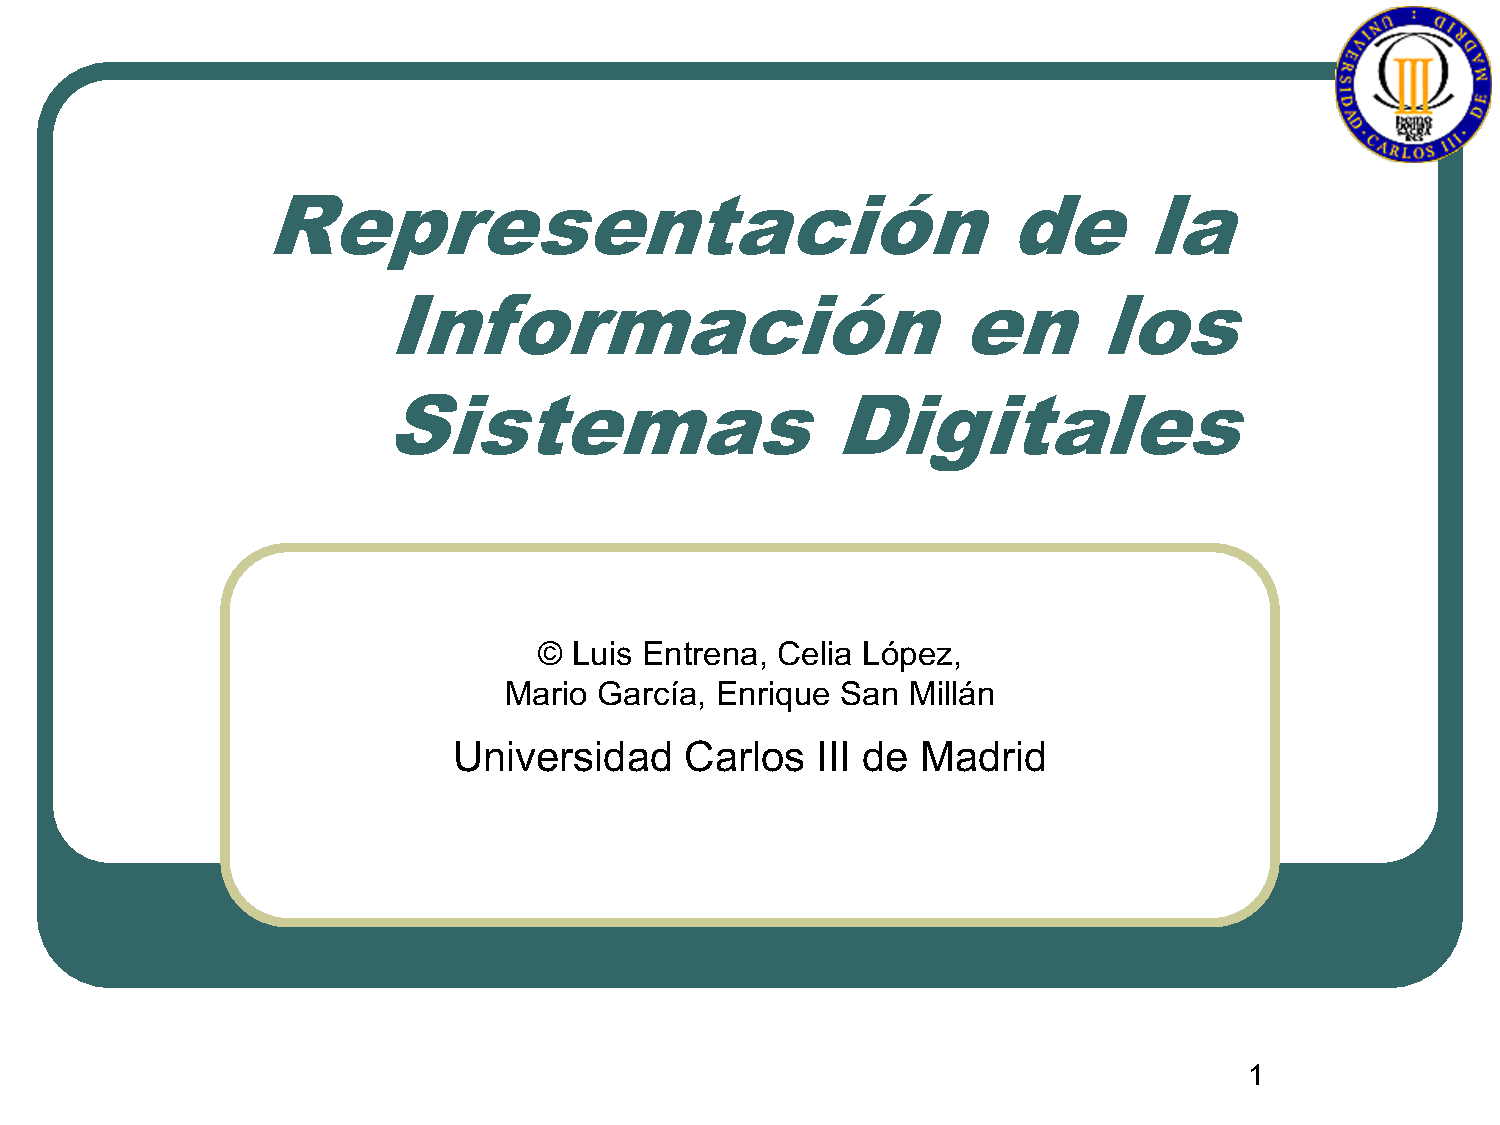
\includepdf[pages=-]{docs/Tema01.Representacion_de_la_informacion.pdf}
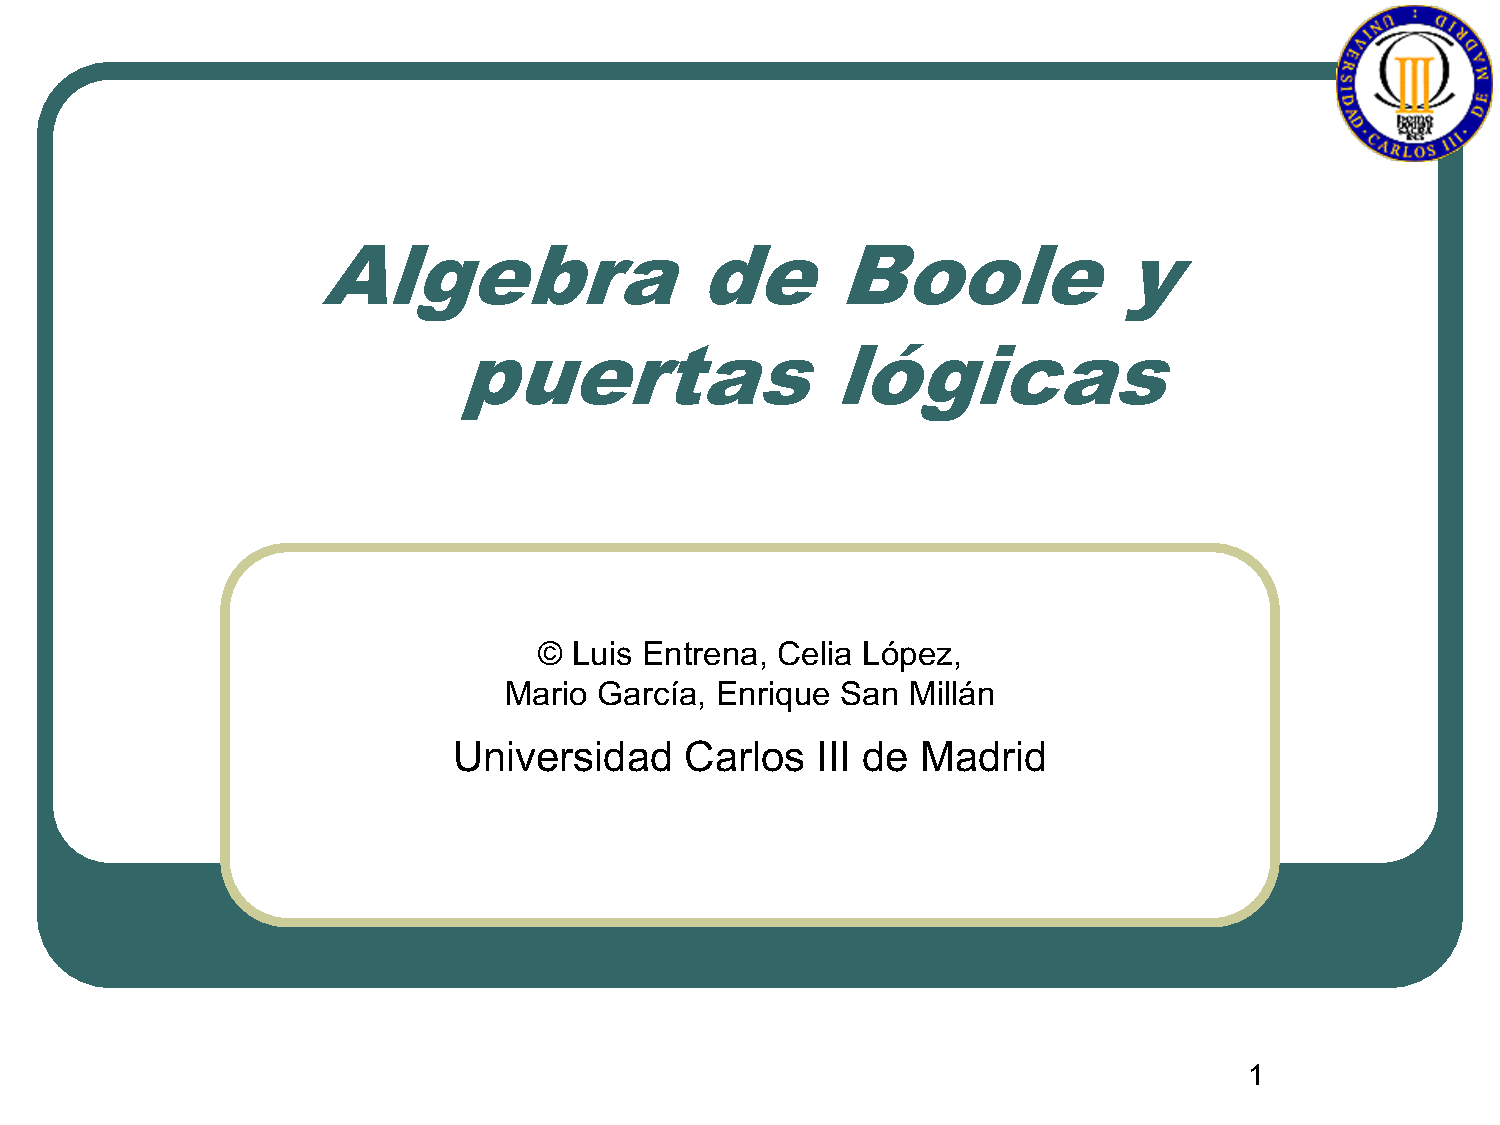
\includepdf[pages=-]{docs/Tema02.Algebra_de_Boole.pdf}
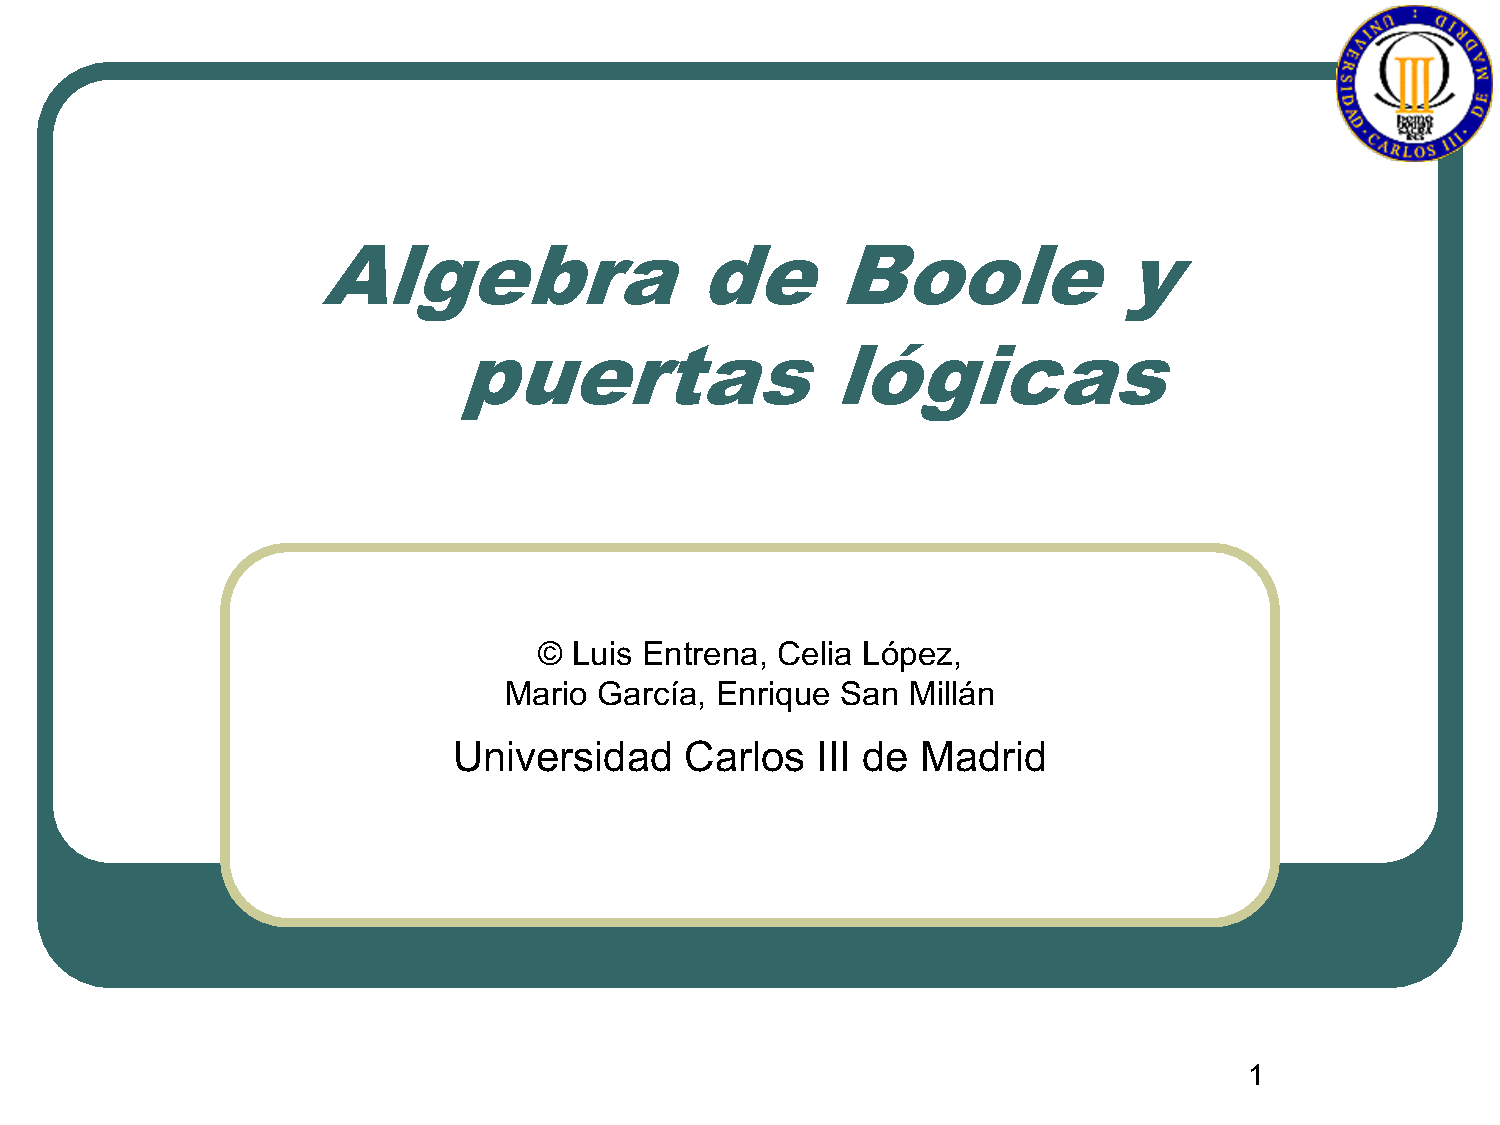
\includepdf[pages=-]{docs/Tema02.Algebra_de_Boole_extra.pdf}
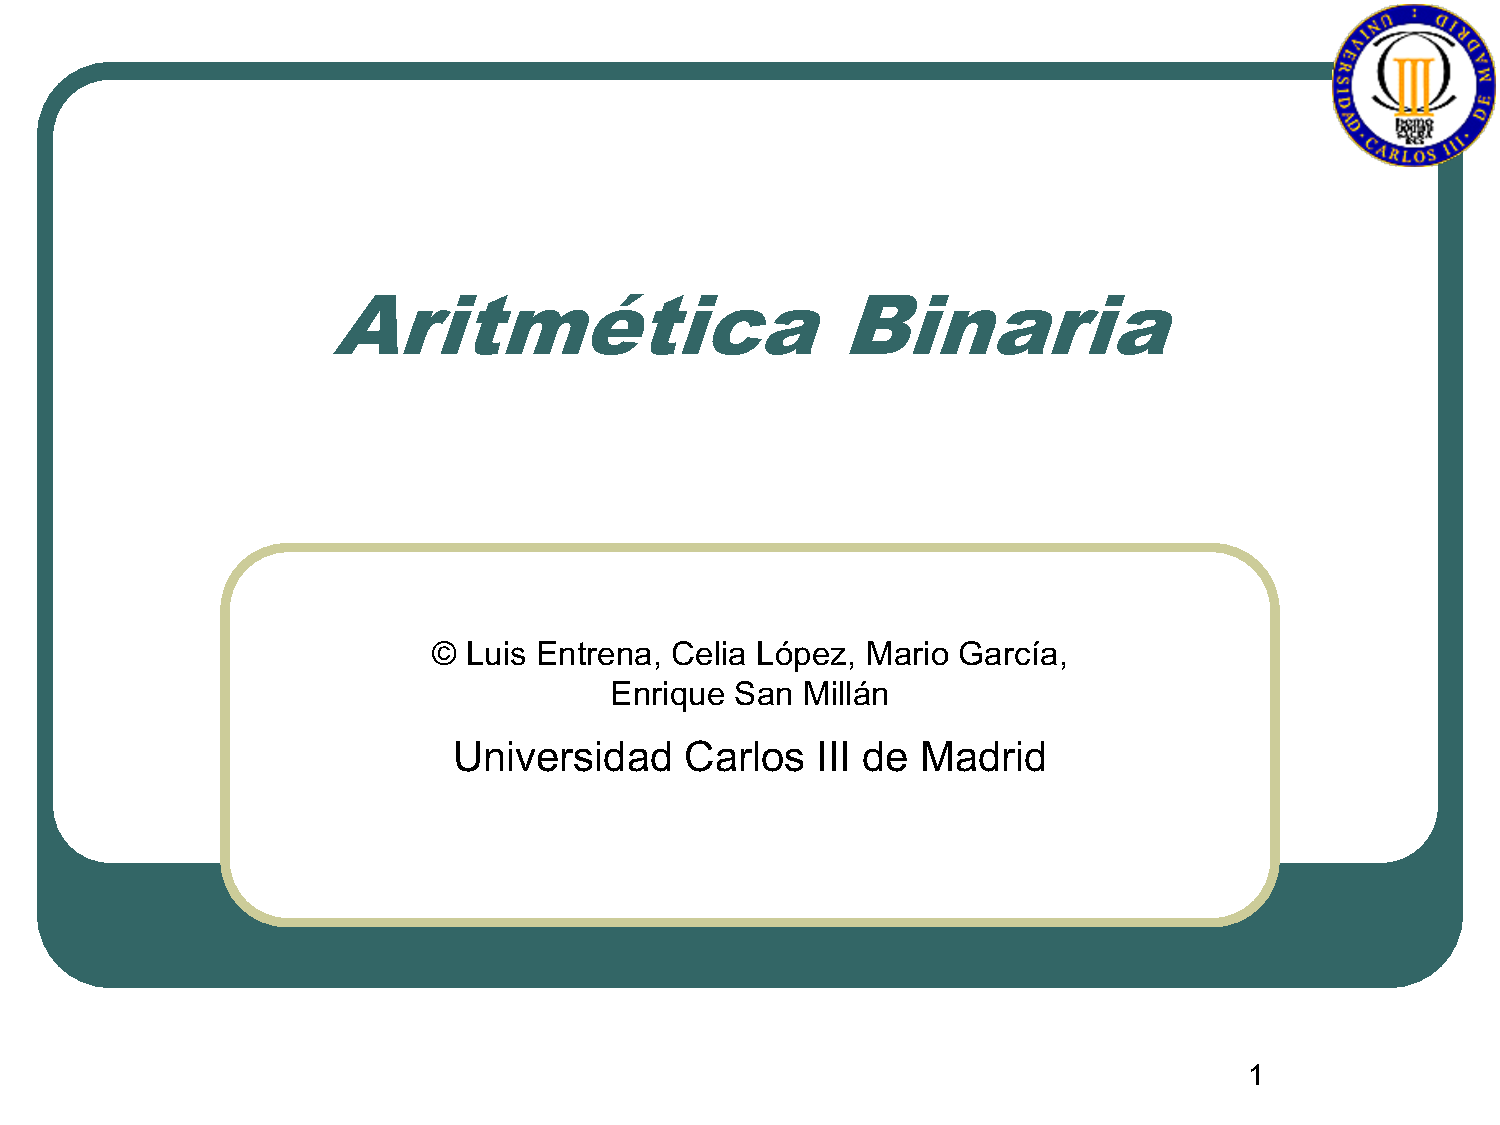
\includepdf[pages=-]{docs/Tema04a.Aritmetica_binaria.pdf}

\includepdf[pages=-]{docs/Tema03.Circuitos_combinacionales.pdf}

\includepdf[pages=-]{docs/Tema04b.Circuitos_combinacionales_aritmeticos_extra.pdf}

\includepdf[pages=-]{docs/Tema06.Circuitos_secuenciales_sincronos.pdf}
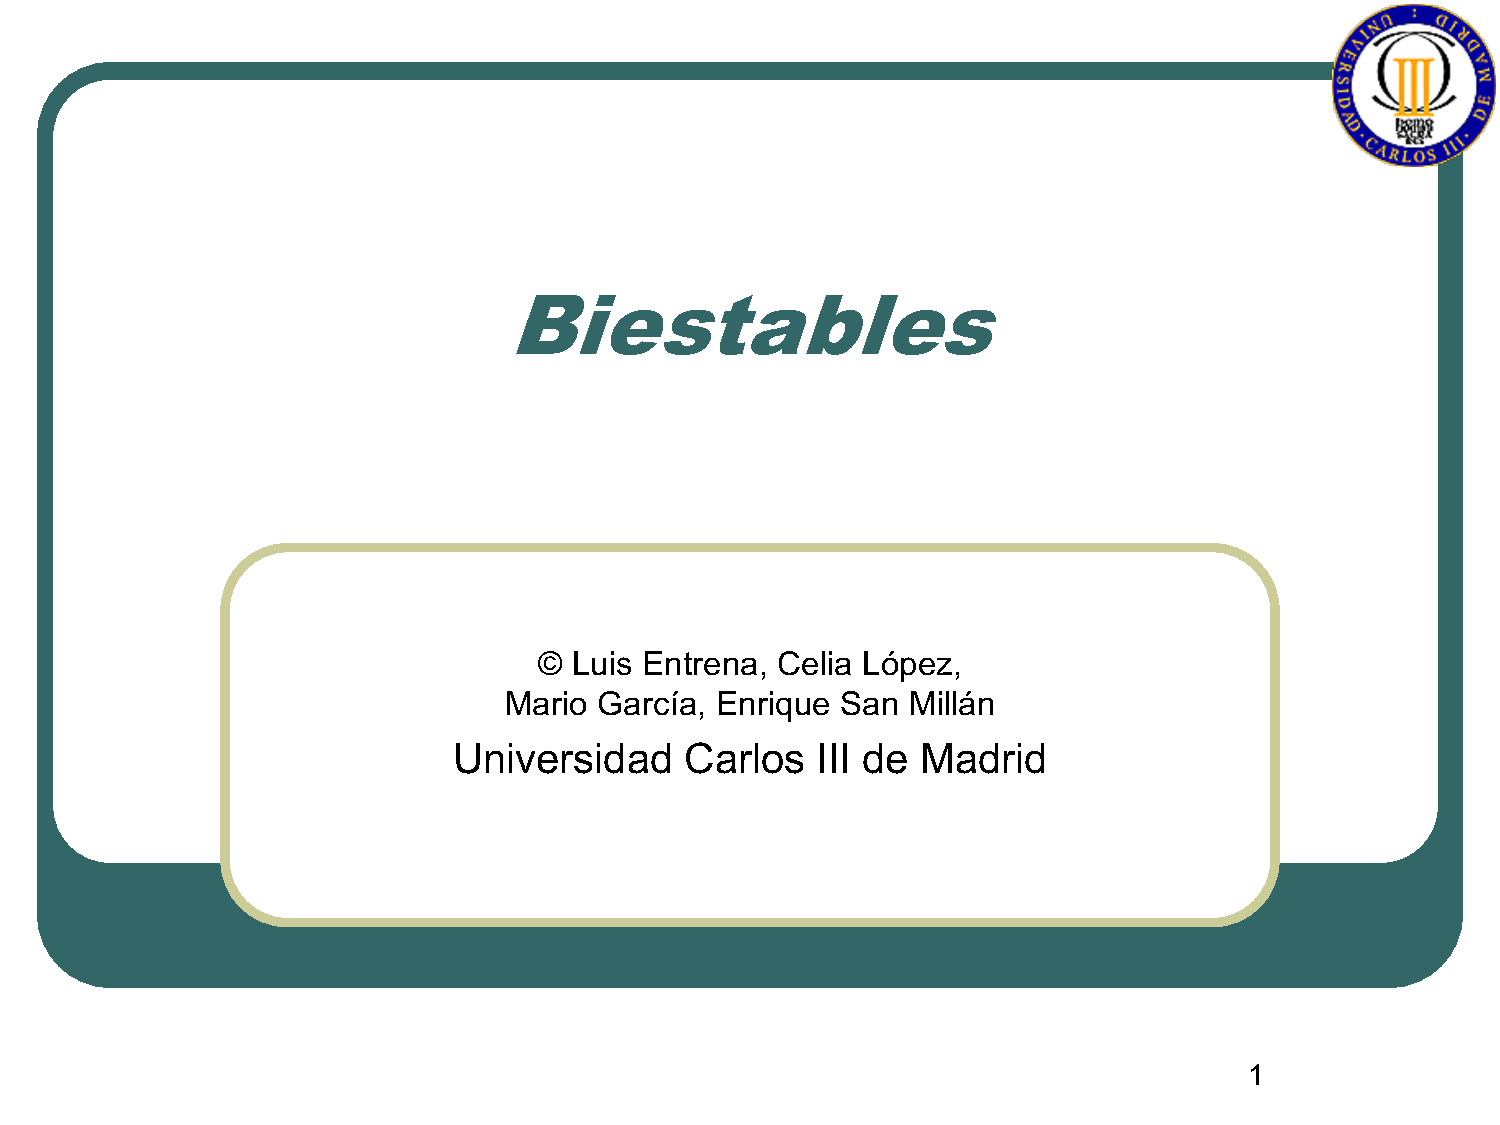
\includepdf[pages=-]{docs/Tema05.Biestables.pdf}

\includepdf[pages=-]{docs/Tema04b.Circuitos_combinacionales_aritmeticos.pdf}
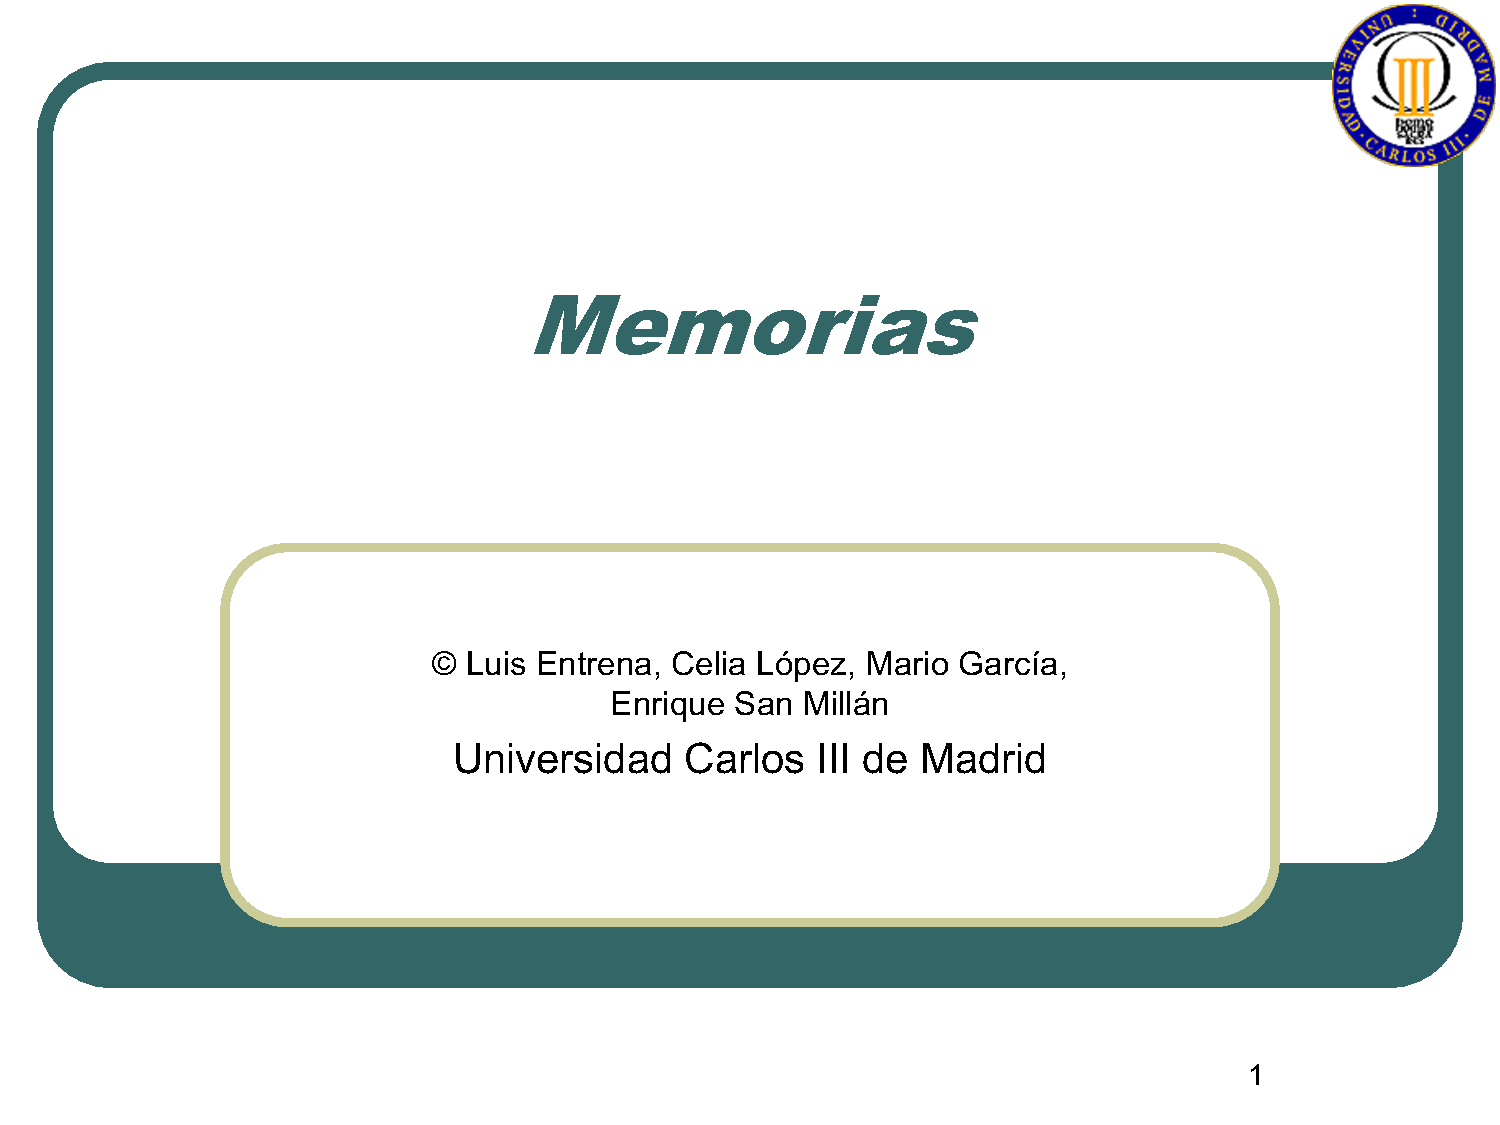
\includepdf[pages=-]{docs/Tema08.Memorias_ampliado.pdf}
\includepdf[pages=-]{docs/Tema07.Registros_y_Contadores.pdf}
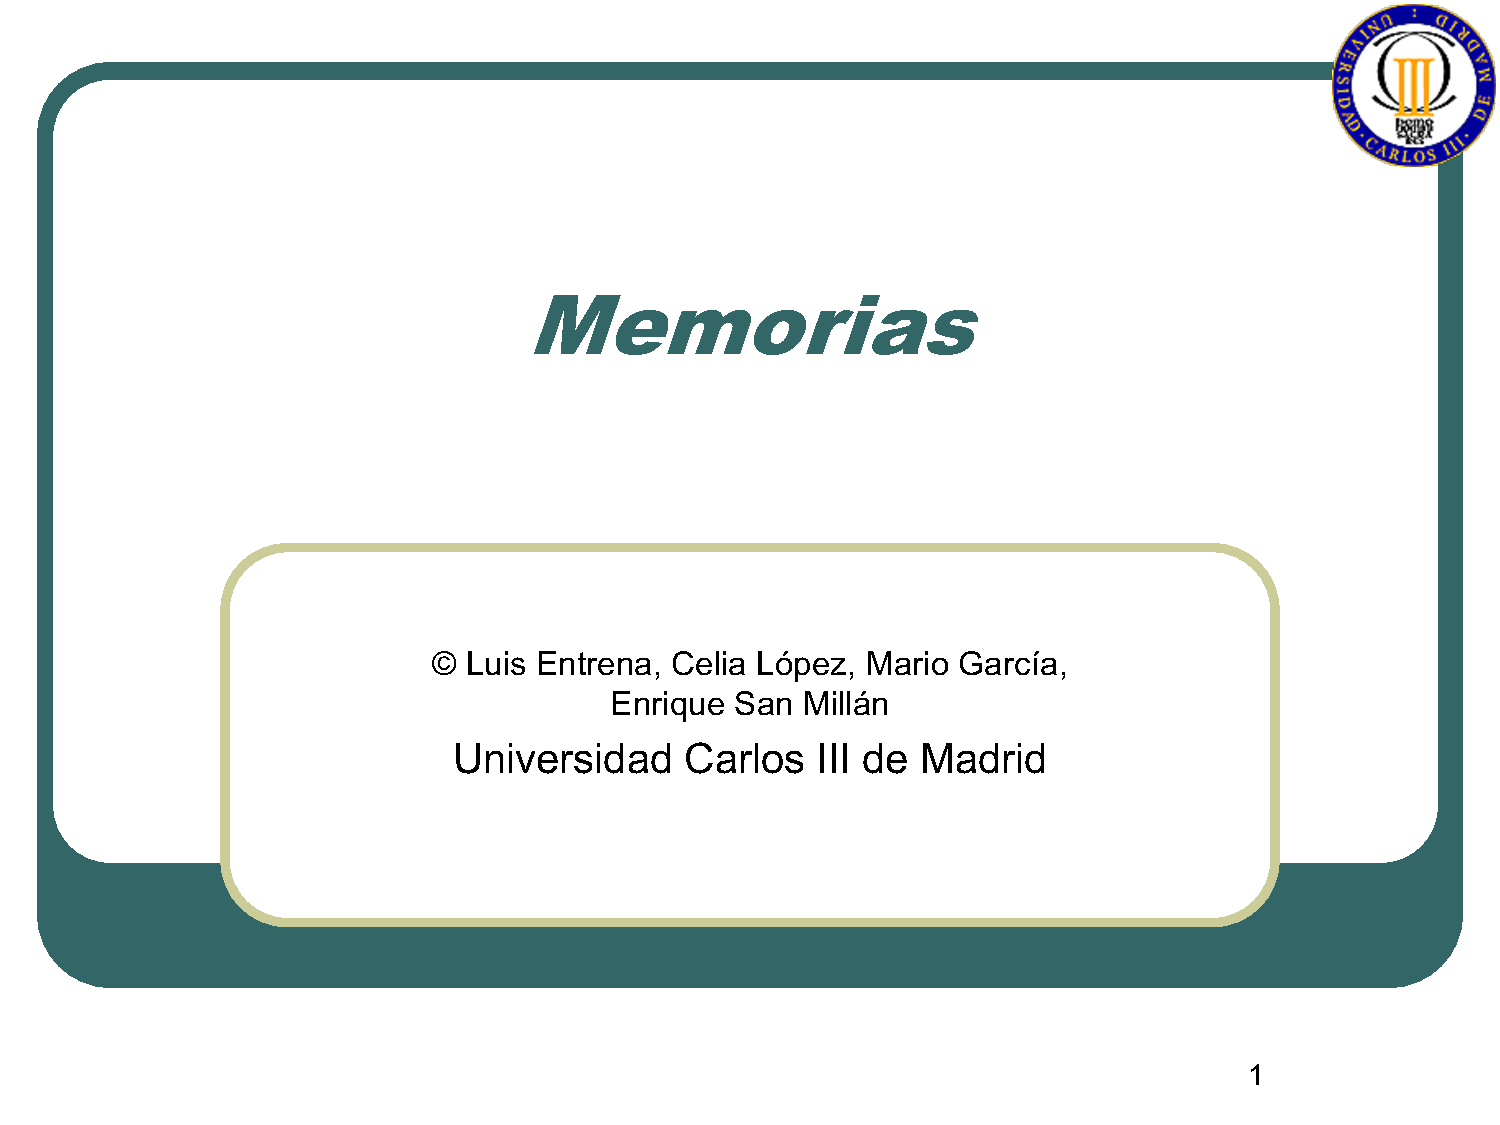
\includepdf[pages=-]{docs/Tema08.Memorias.pdf}
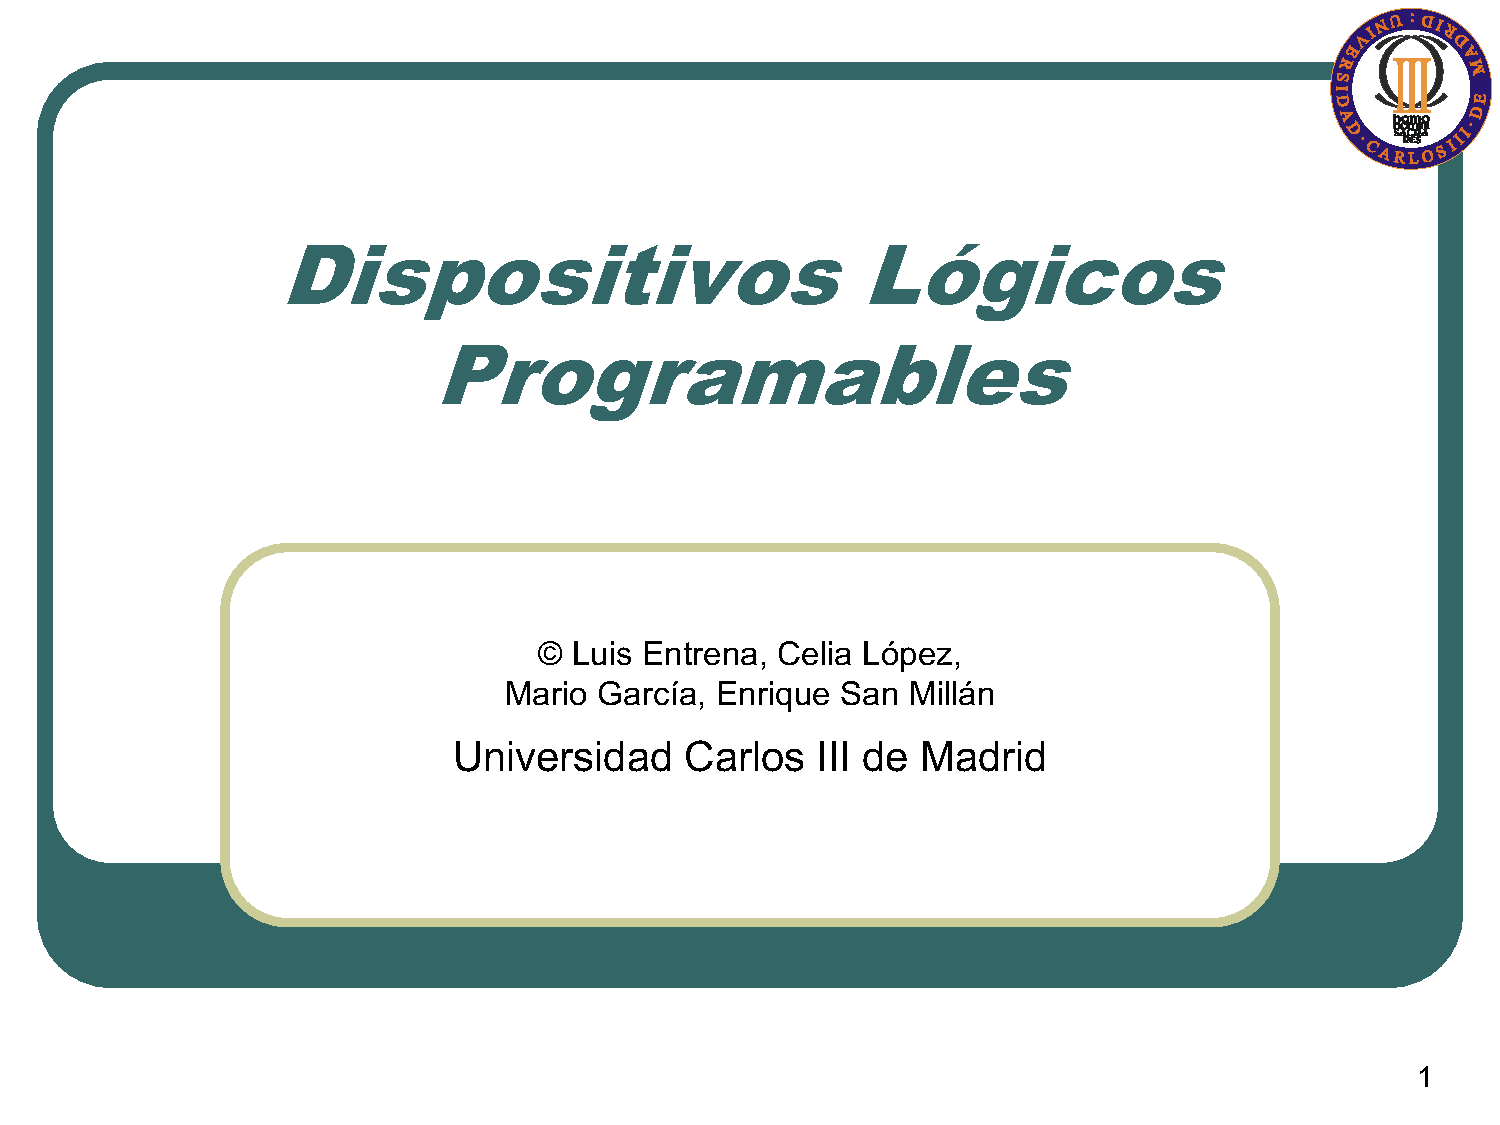
\includepdf[pages=-]{docs/Tema09.Dispositivos_logicos_programables.pdf}
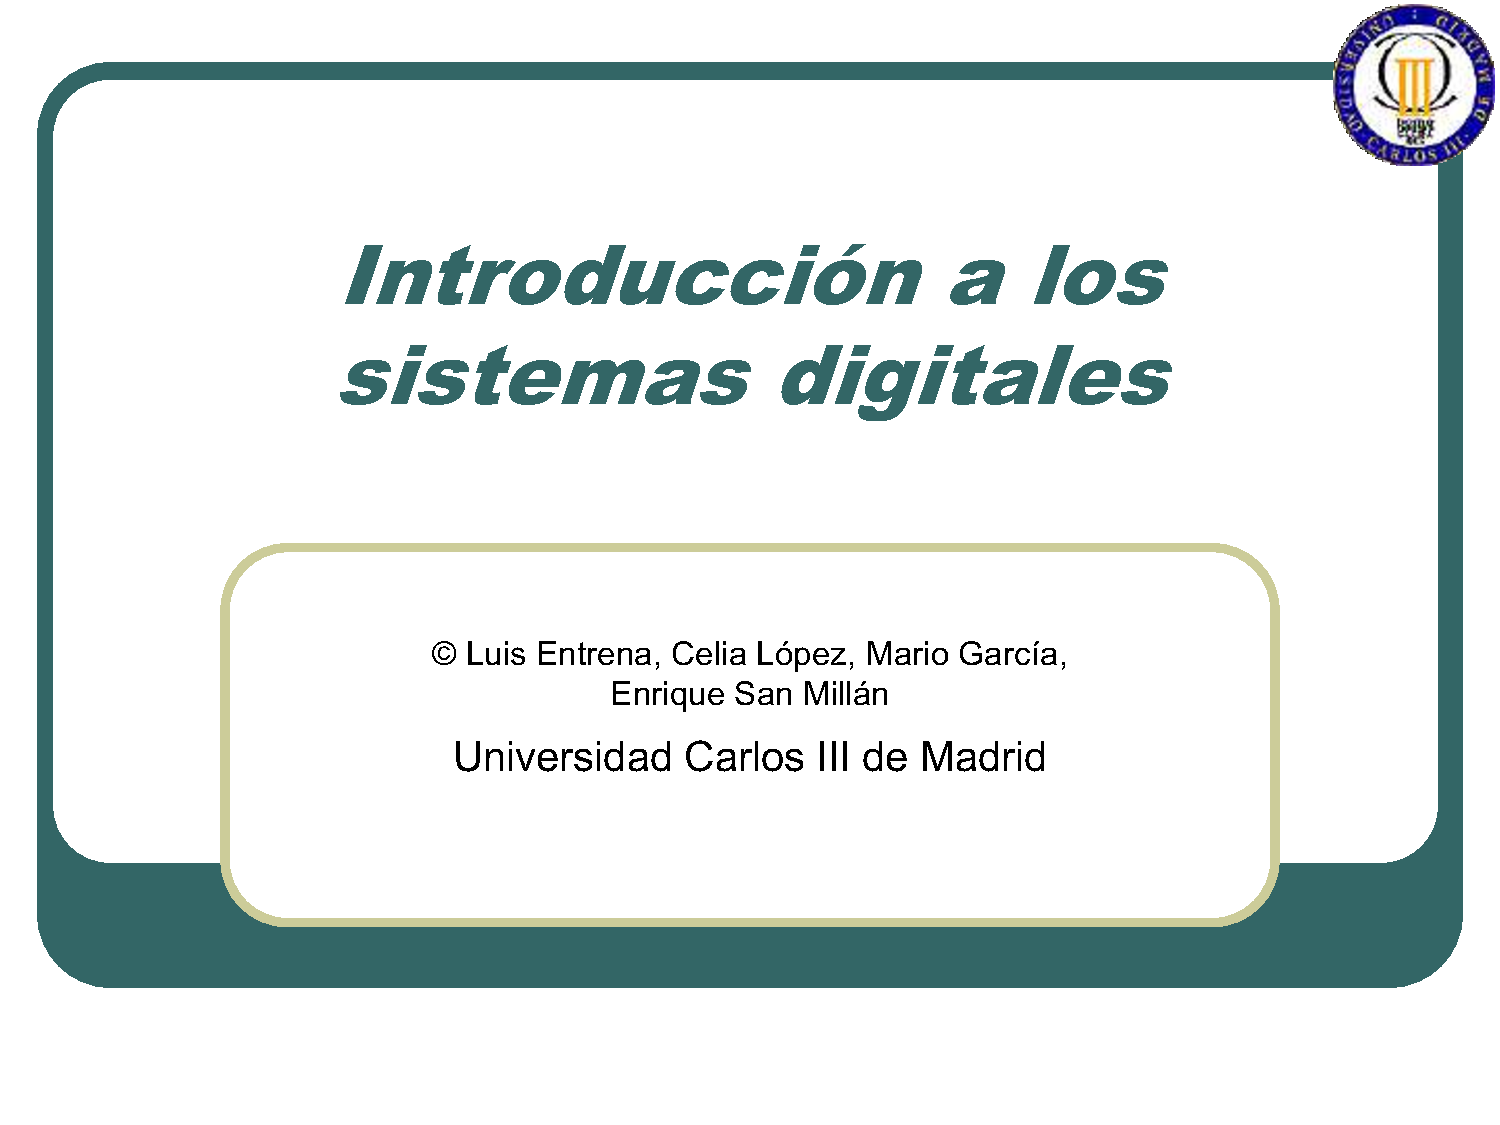
\includepdf[pages=-]{docs/Tema10.Sistemas_digitales_rev2013.pdf}


\part{Problemas}
\includepdf[pages=-]{docs/TC_Combinaciona_sol.pdf}
\includepdf[pages=-]{docs/TC_Combinacional_eng.pdf}
\includepdf[pages=-]{docs/TC_Combinacional.pdf}
\includepdf[pages=-]{docs/PROBLEMAS_Propuestos_Biestables_Cronogramas_Eng_bis.pdf}
\includepdf[pages=-]{docs/PROBLEMAS_Propuestos_Biestables_Cronogramas_Esp.pdf}
\includepdf[pages=-]{docs/PROBLEMAS_Resueltos_Biestables_Cronogramas_Eng_bis.pdf}
\includepdf[pages=-]{docs/PROBLEMAS_Resueltos_Biestables_Cronogramas_Esp.pdf}
\includepdf[pages=-]{docs/S8_Memorias_enunciado_sol_eng.pdf}
\includepdf[pages=-]{docs/S9_Memorias_enunciado_sol_eng.pdf}
\includepdf[pages=-]{docs/Soluciones_Prob_tema2_TC_ITIG_2.pdf}
\includepdf[pages=-]{docs/TC_Arith_sol.pdf}
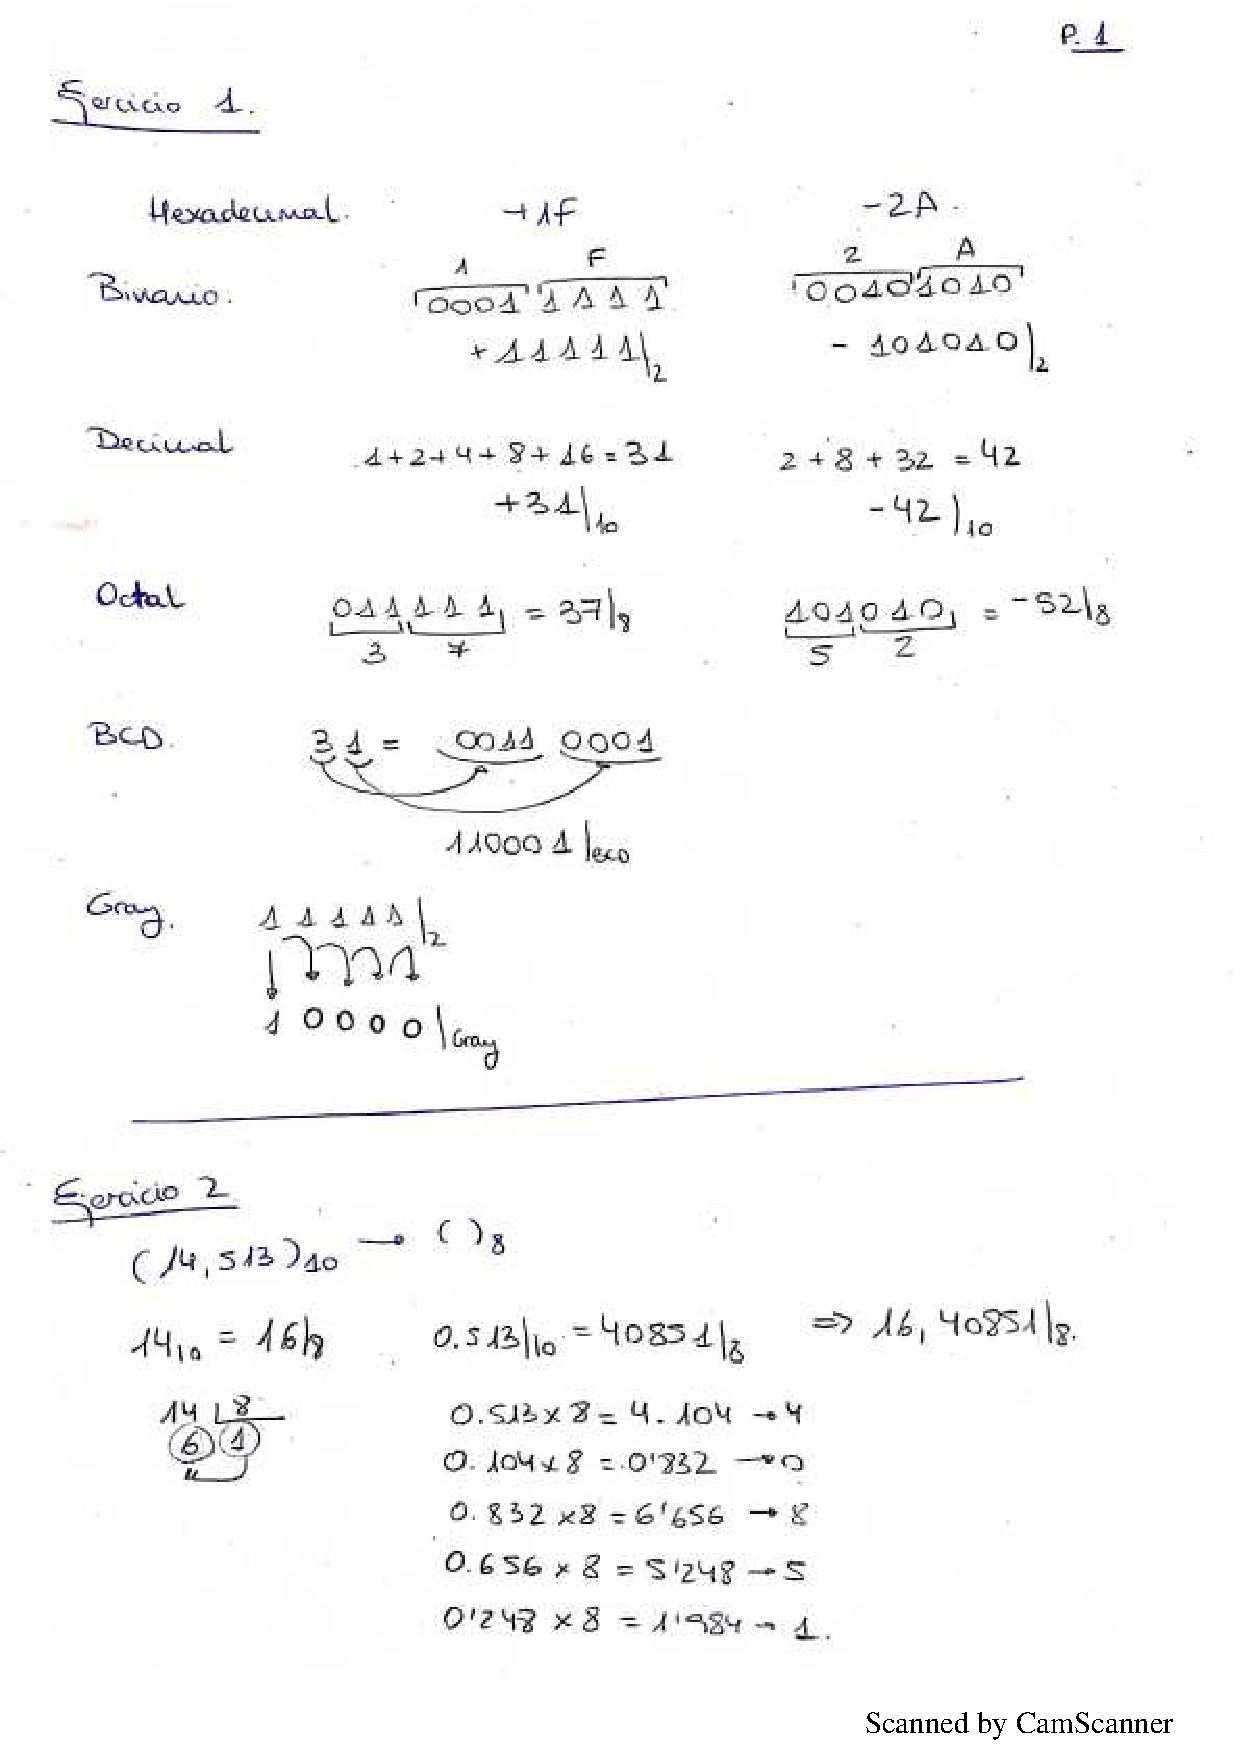
\includepdf[pages=-]{docs/TC_Boole_y_sistemas_de_numeracion_sol_a_mano.pdf}
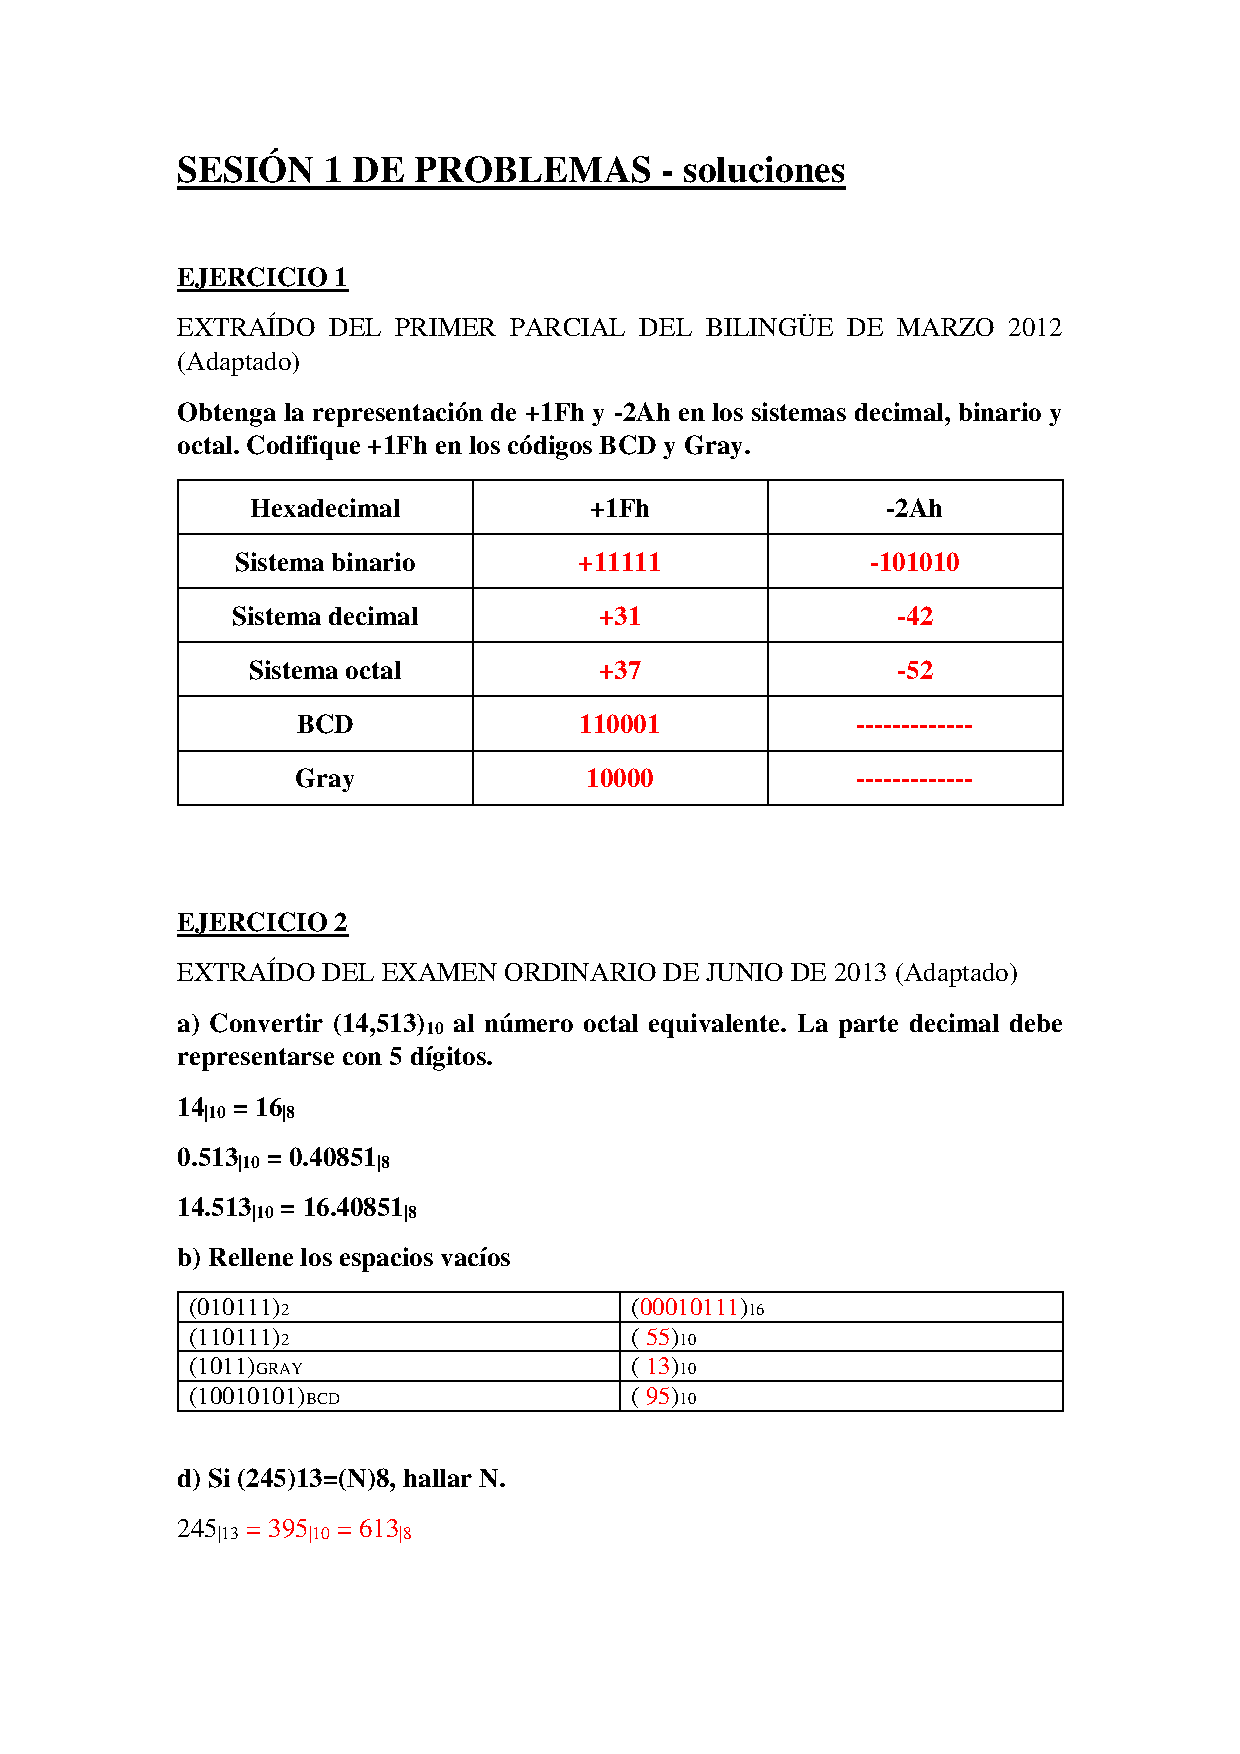
\includepdf[pages=-]{docs/TC_Boole_y_sistemas_de_numeracion_sol.pdf}

\part{Sesión 1}

\includepdf[pages=-]{docs/1819TC_ManualPracticas_PR1_2.pdf}
\includepdf[pages=-]{docs/mae-jrf-MemoriaSesion1.pdf}

\part{Sesión 2}

\includepdf[pages=-]{docs/1819TC_ManualPracticas_PR1_2.pdf}
\includepdf[pages=-]{docs/mae-jrf-MemoriaSesion2.pdf}
\includepdf[pages=-]{docs/mae-jrf-MemoriaSesion2.pdf}

\part{Sesión 3}
\includepdf[pages=-]{docs/1819TC_ManualPracticas_PR3.pdf}
\includepdf[pages=-]{docs/PDFmae-jrf-MemoriaSesion3.pdf}
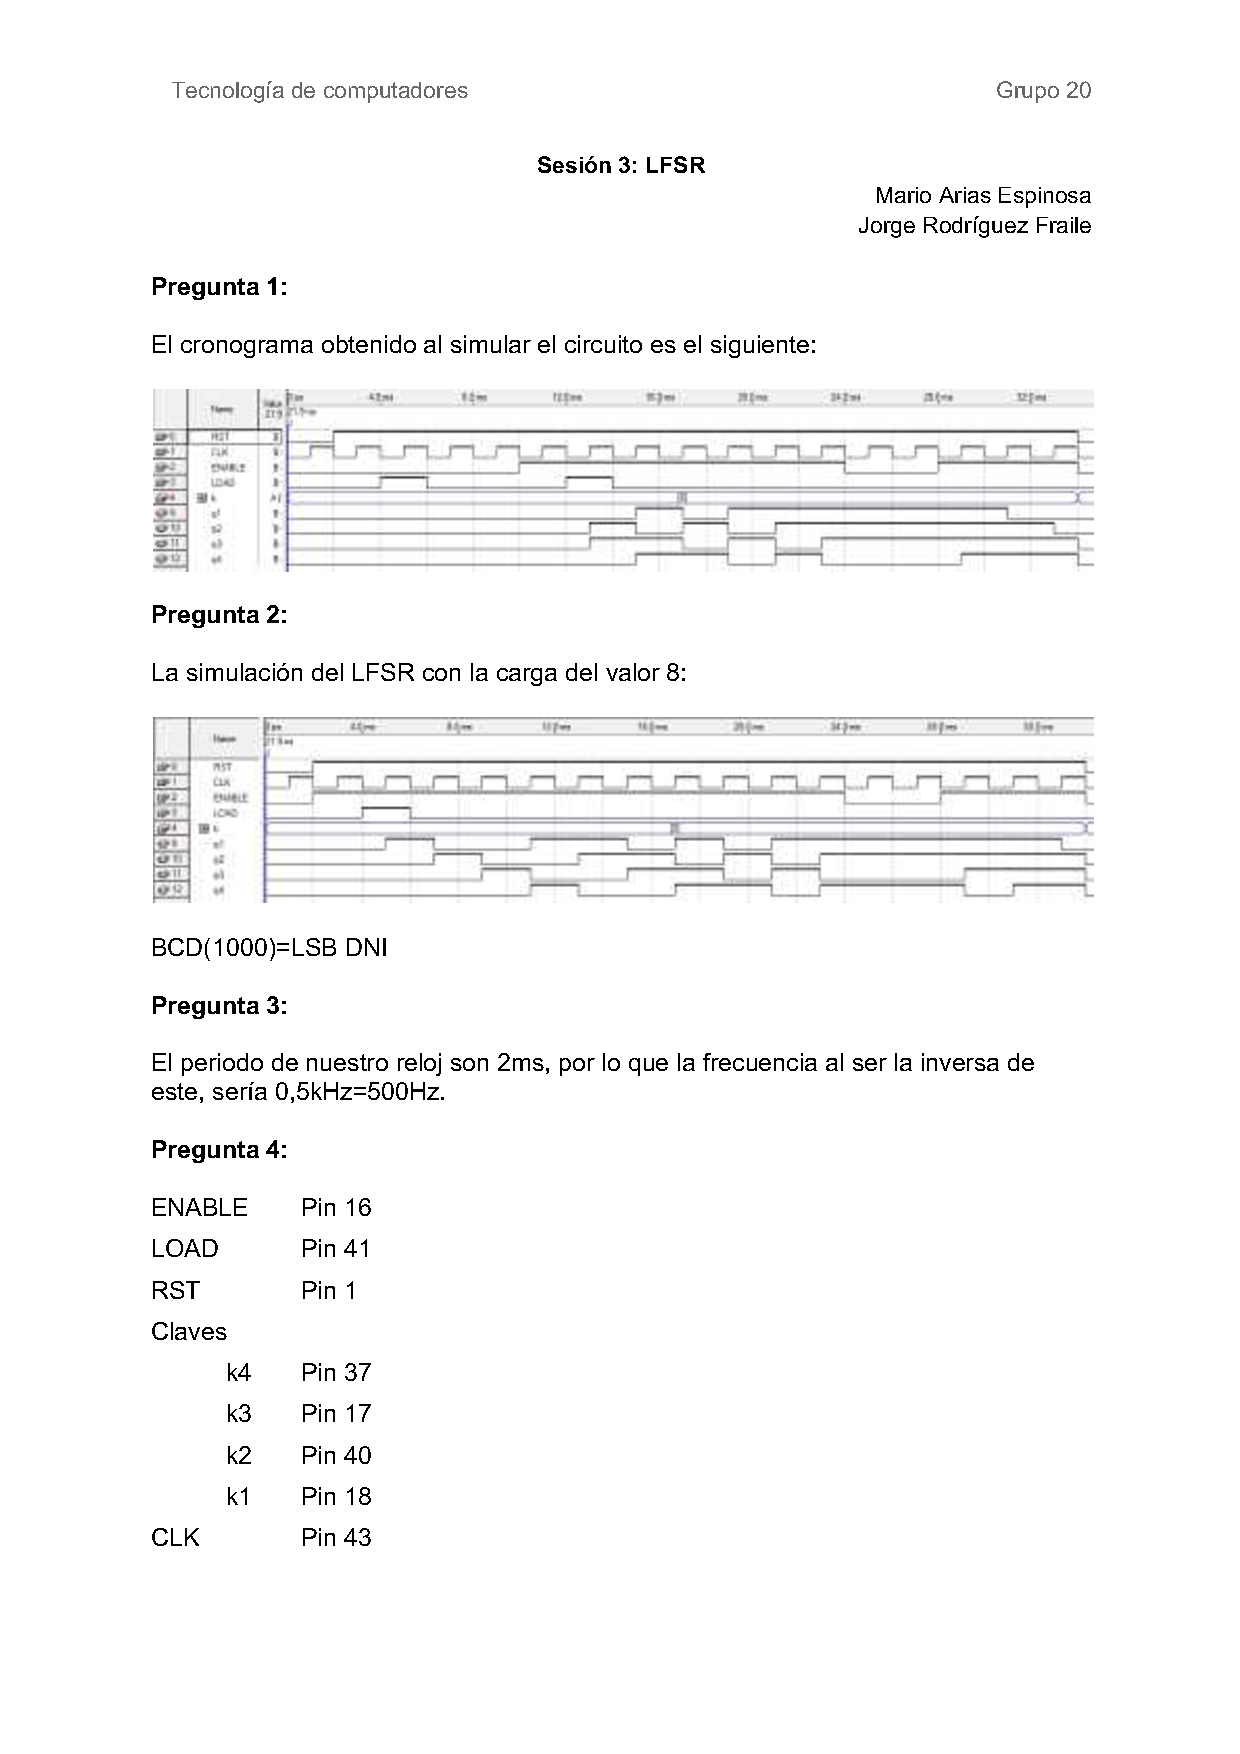
\includepdf[pages=-]{docs/mae-jrf-MemoriaSesion3.pdf}

\part{Sesión 4}
\includepdf[pages=-]{docs/1819TC_ManualPracticas_PR4.pdf}
\includepdf[pages=-]{docs/PDFmae-jrf-MemoriaSesion4.pdf}
\includepdf[pages=-]{docs/mae-jrf-MemoriaSesion4.pdf}

\part{Examenes}
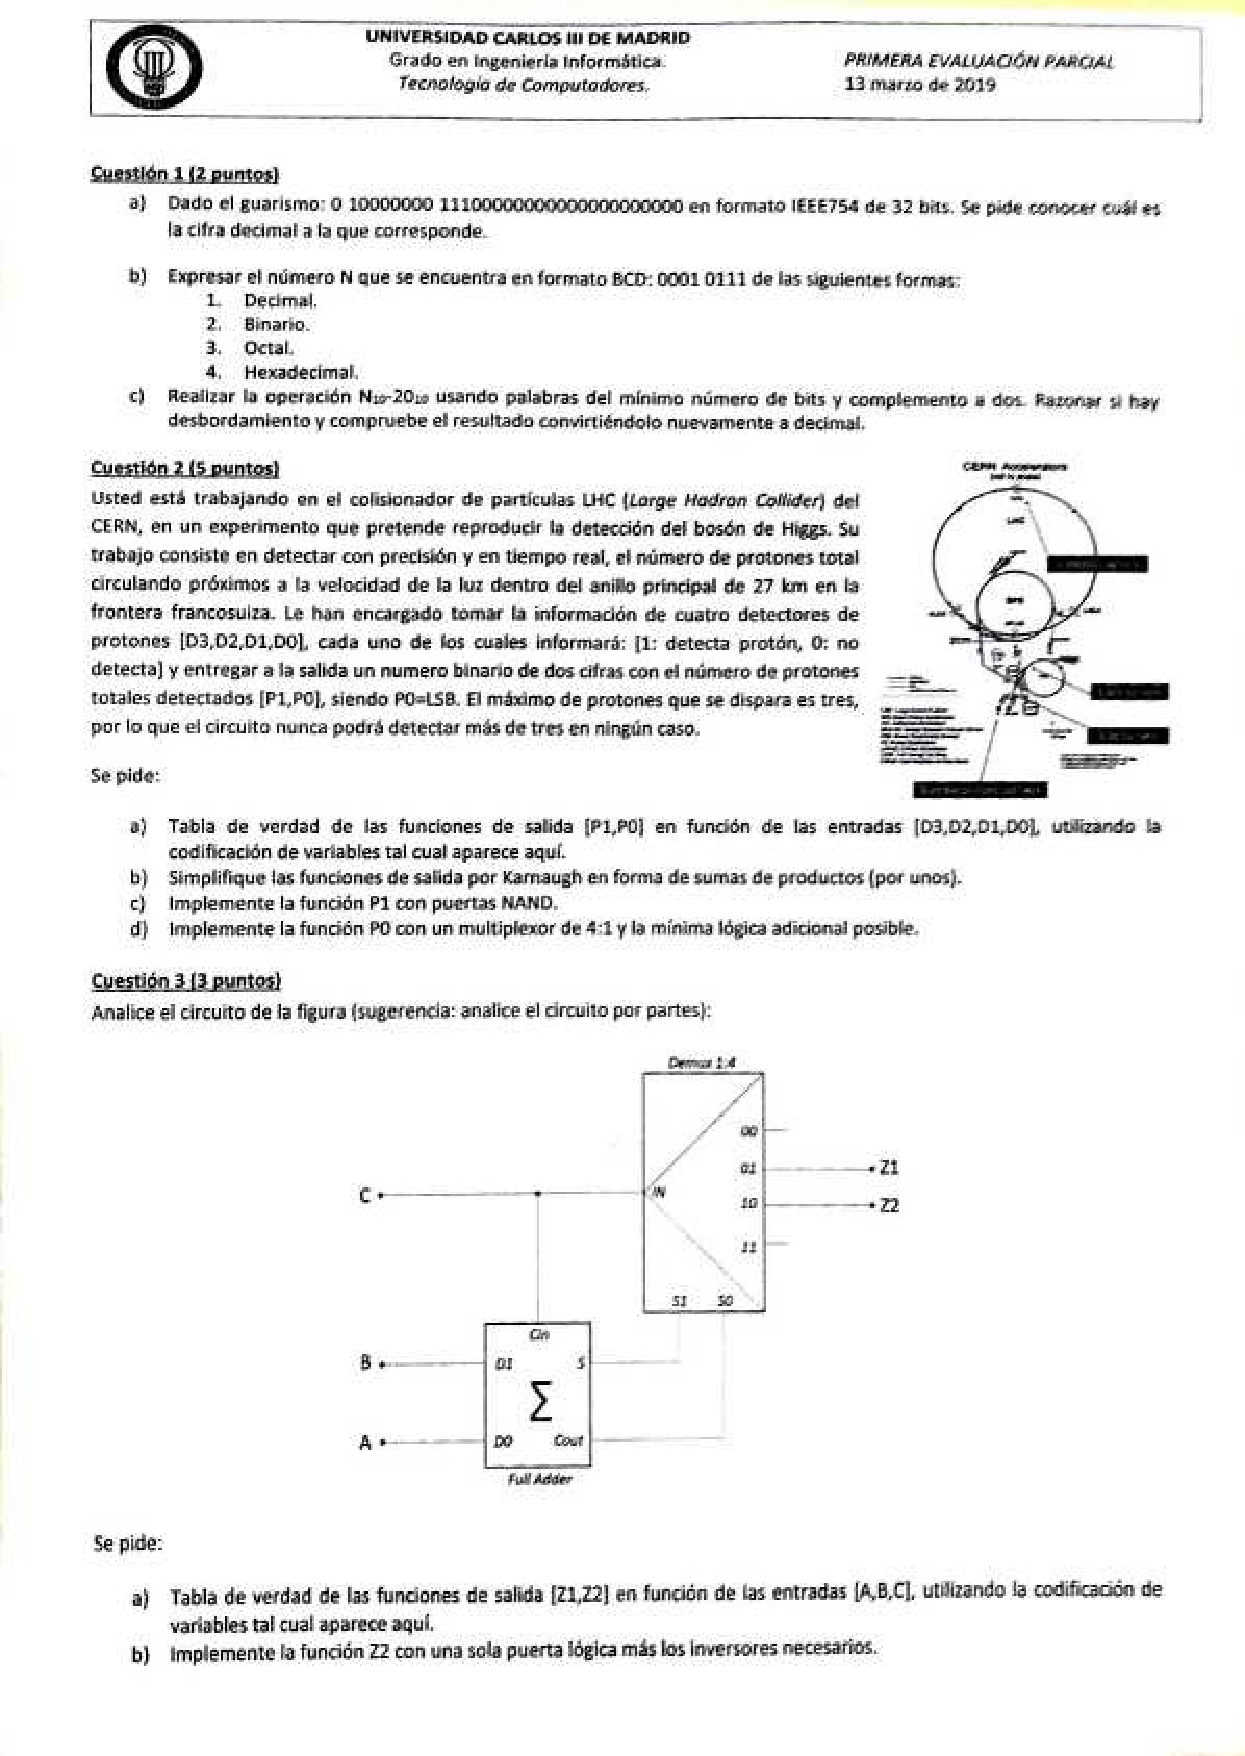
\includepdf[pages=-]{docs/TC_Parcial_1_Marzo_2019.pdf}
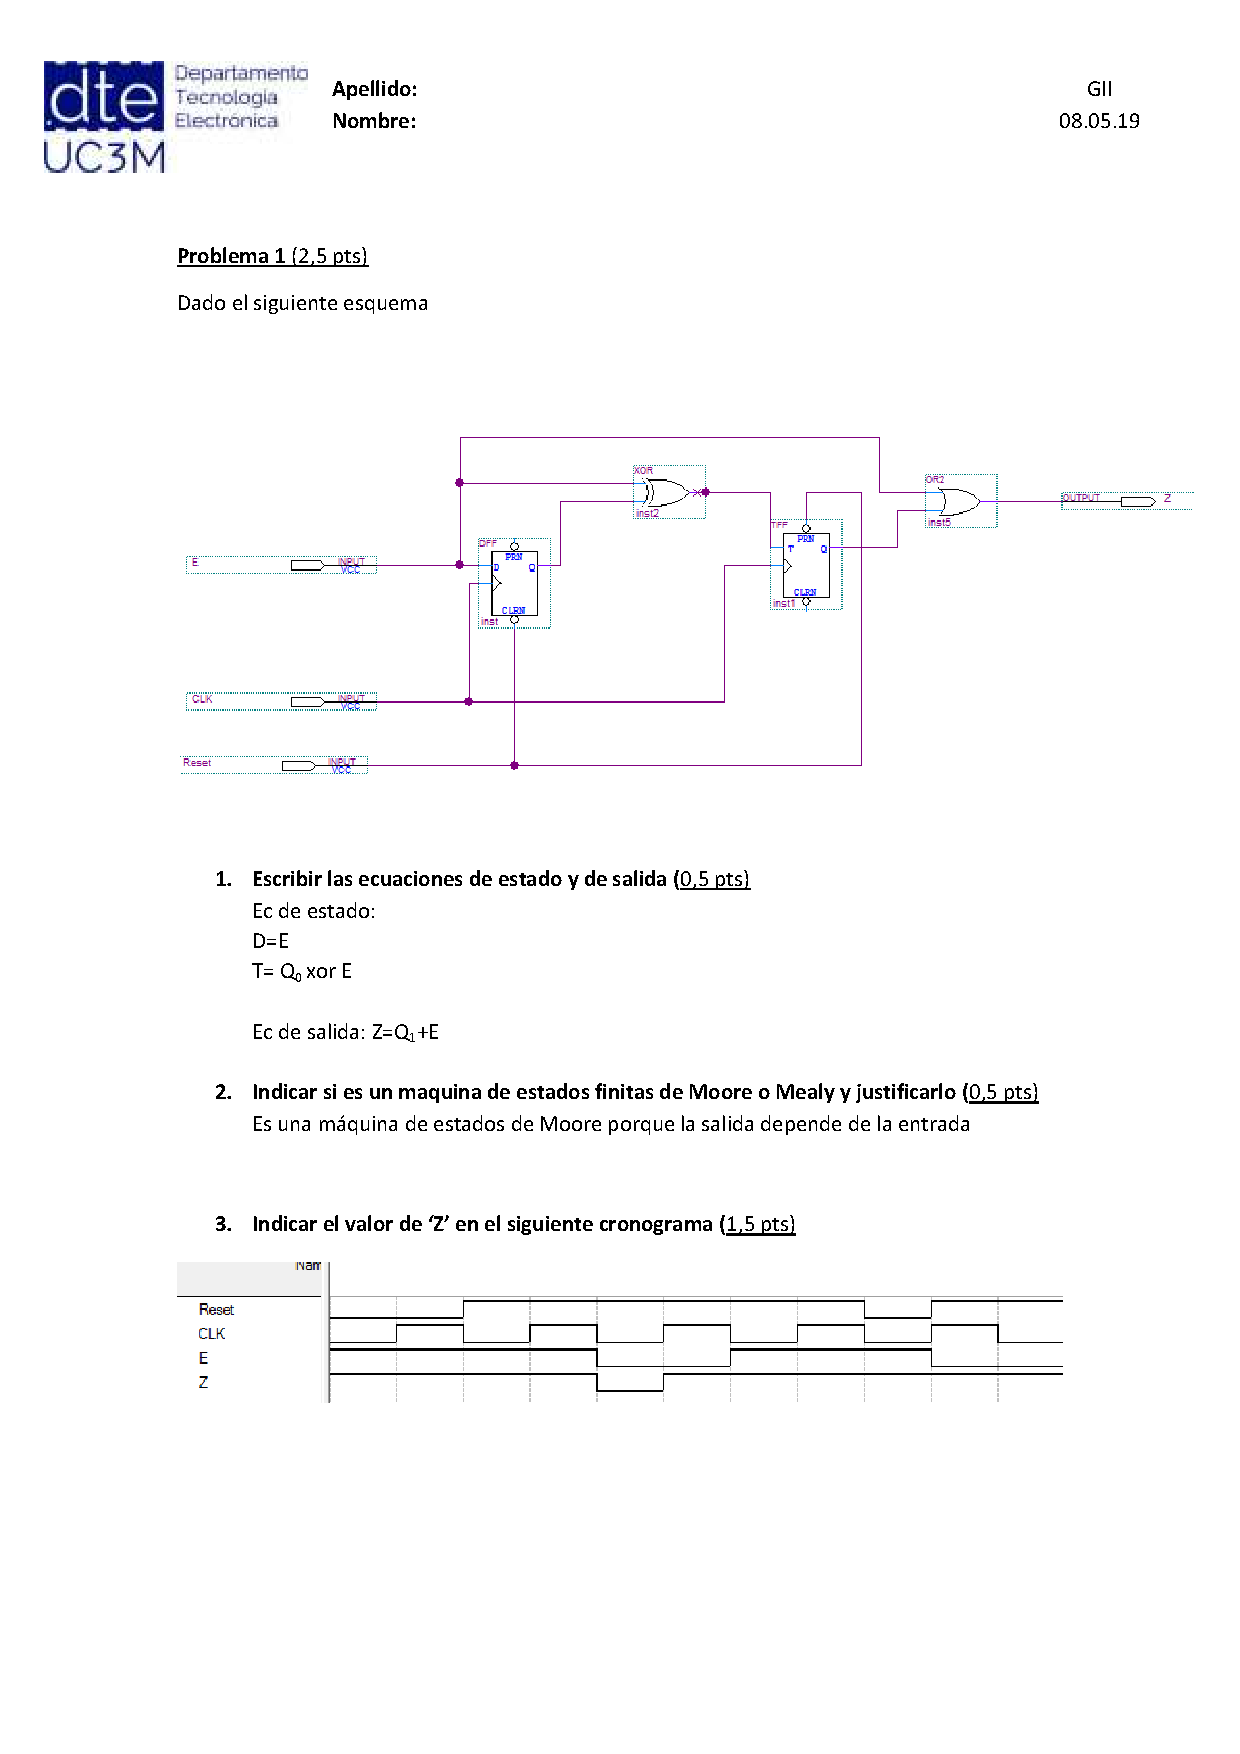
\includepdf[pages=-]{docs/TC_2P_G_84_18_19_v_solucion.pdf}
\includepdf[pages=-]{docs/2013_2014_4_Make_Up_Exam_Solution_1_and_4.pdf}
\includepdf[pages=-]{docs/1718TC_First-midterm-exam_GR88_89.pdf}
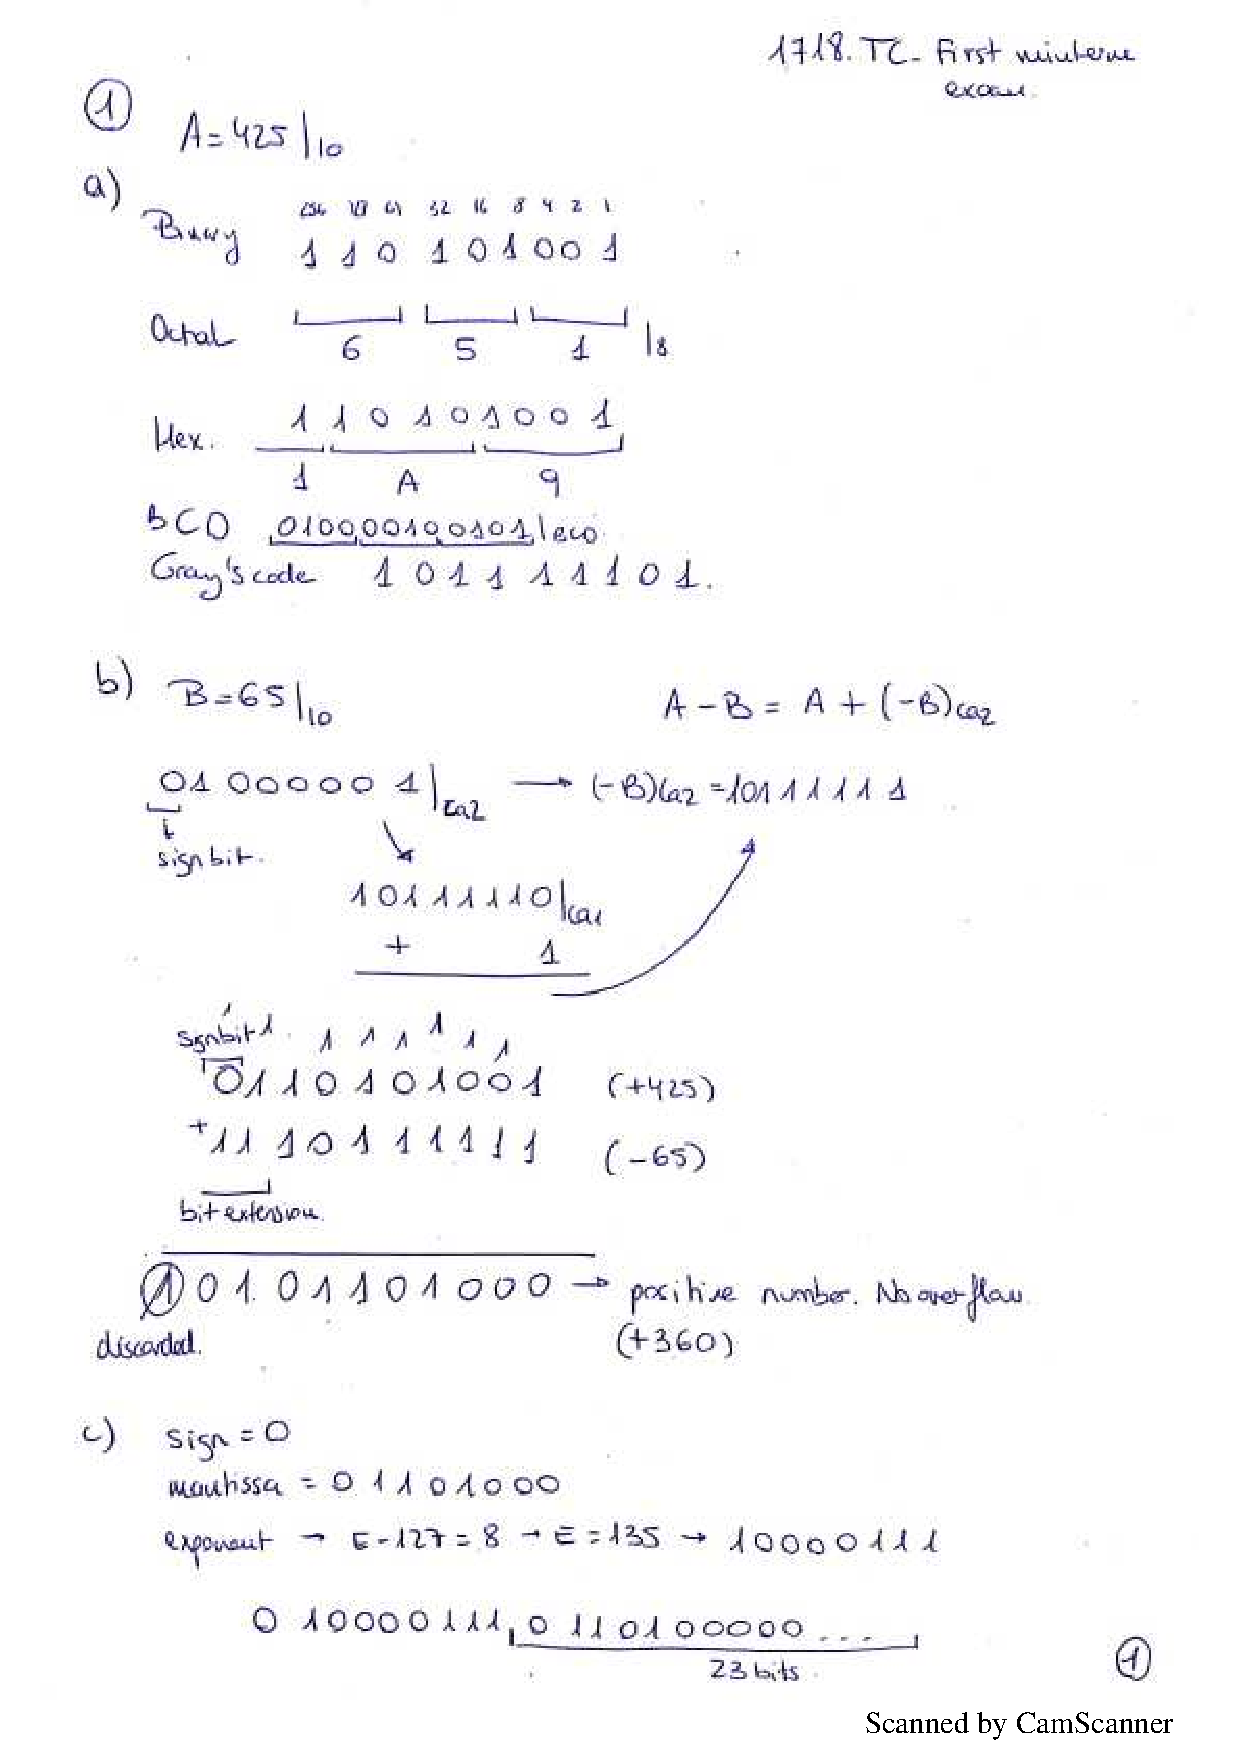
\includepdf[pages=-]{docs/1718TC_First-midterm-exam-solutions.pdf}
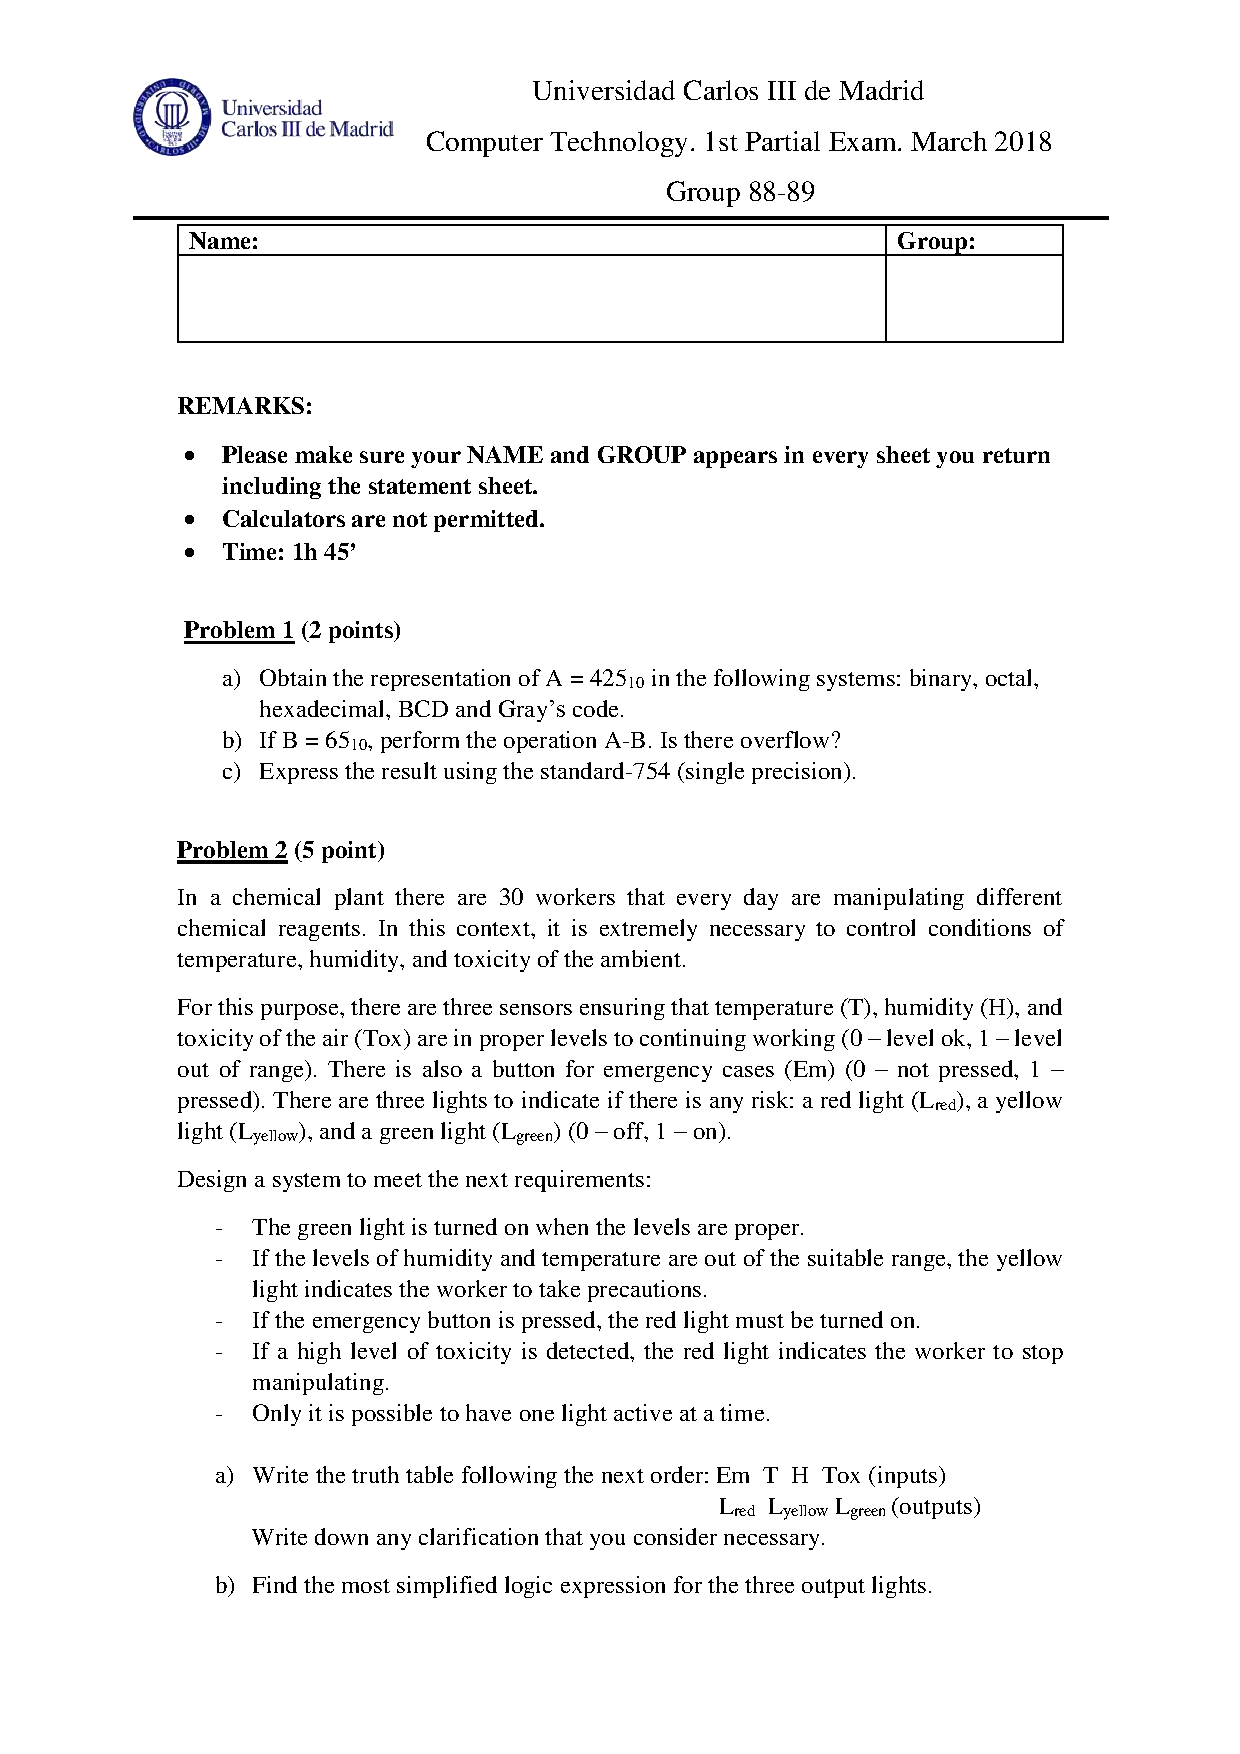
\includepdf[pages=-]{docs/1718TC_First-midterm-exam.pdf}
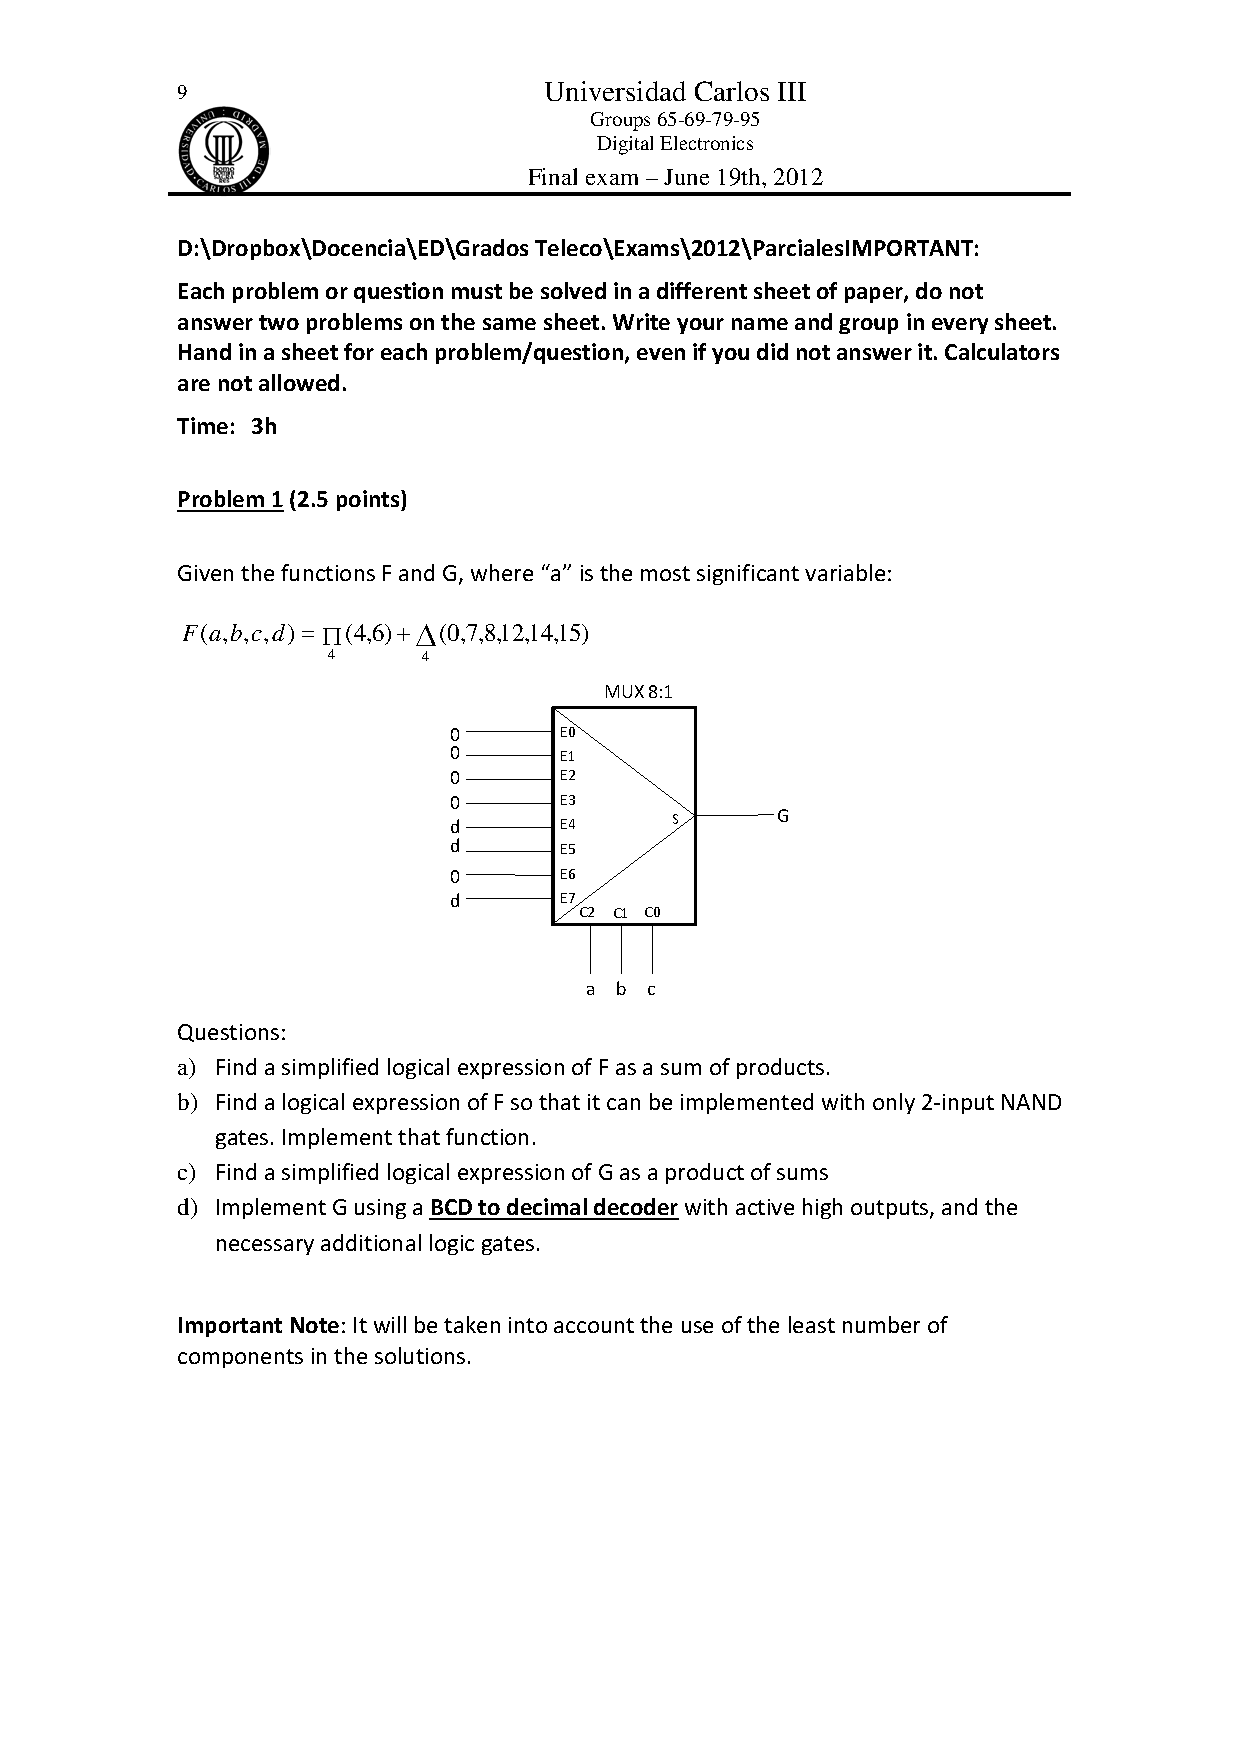
\includepdf[pages=-]{docs/2012_Final_Exam_Solutions.pdf}
\includepdf[pages=-]{docs/2012_First_Midterm_Exam_Solution.pdf}
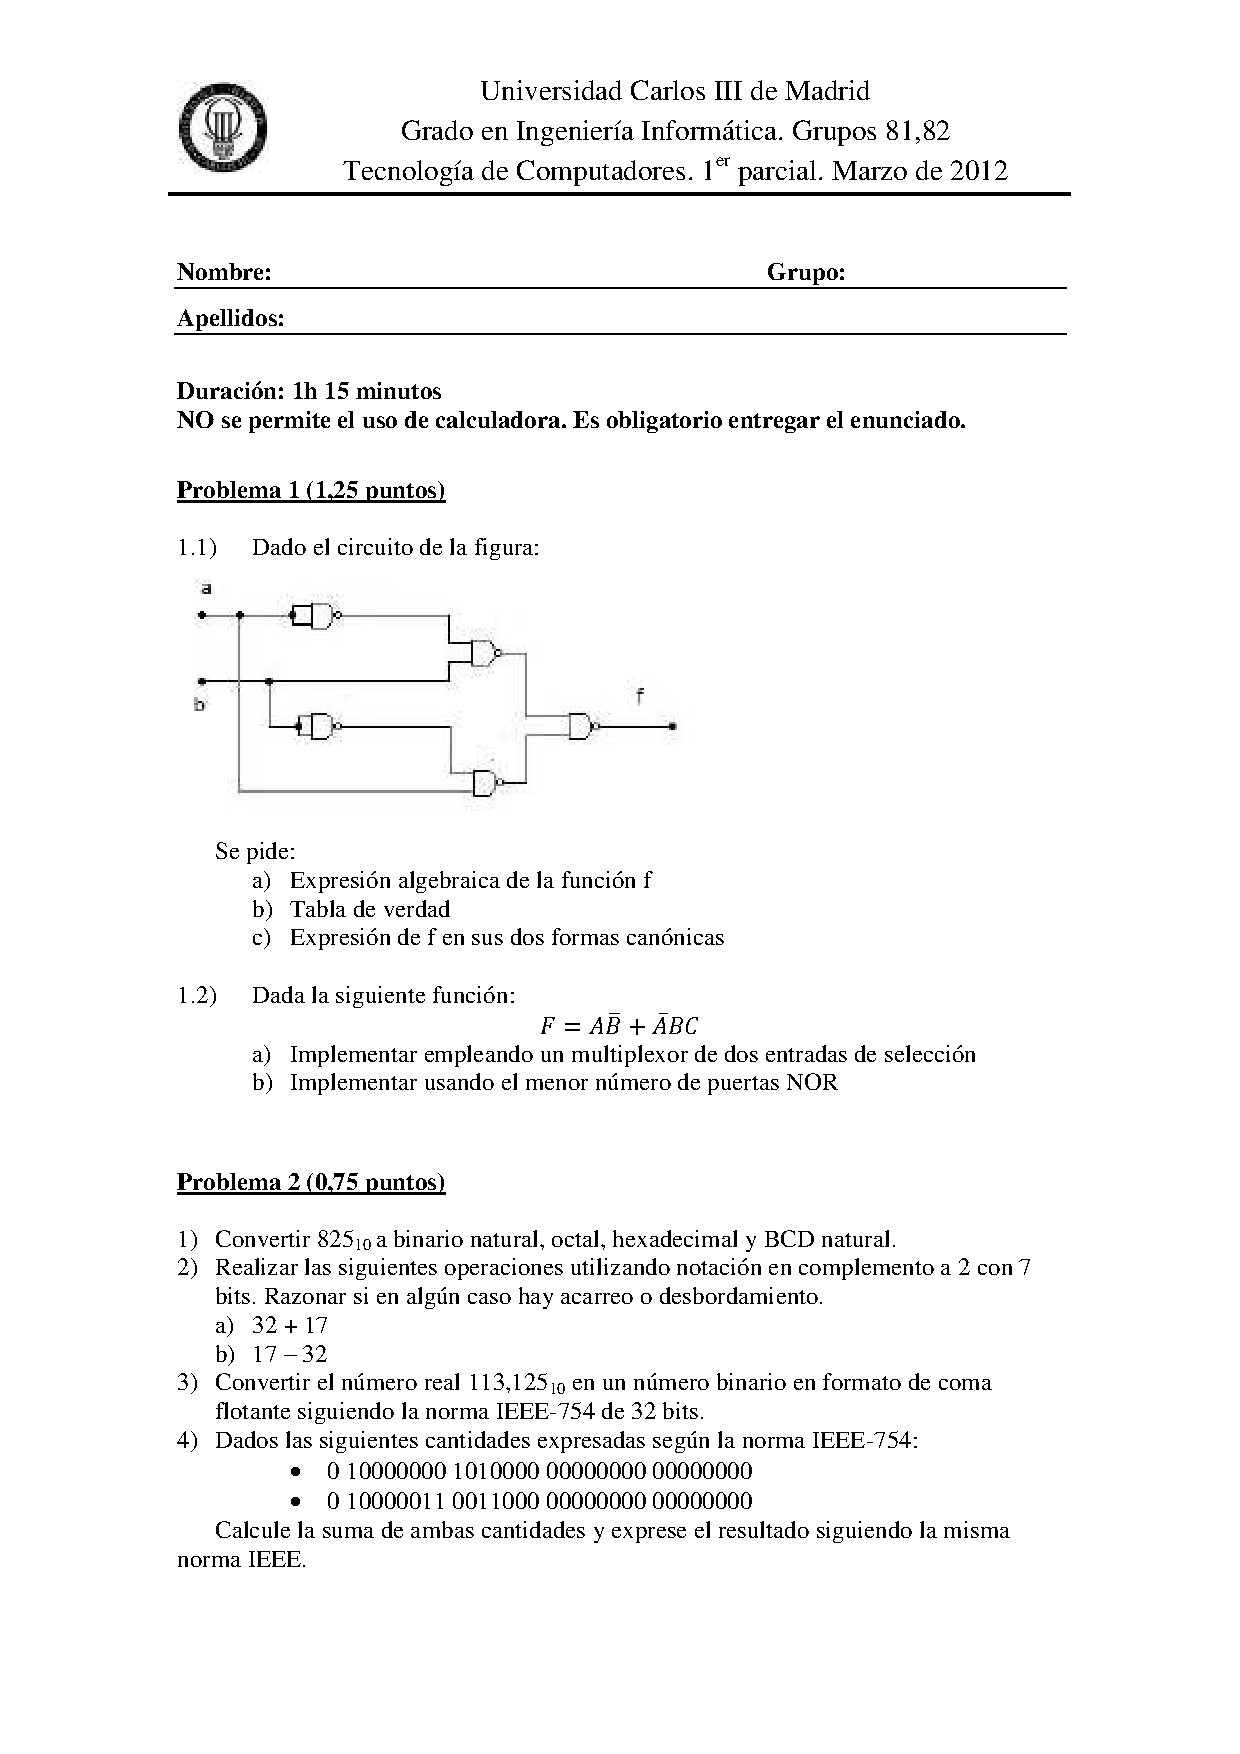
\includepdf[pages=-]{docs/2012_Primer_Parcial_Examen_Soluciones.pdf}
\includepdf[pages=-]{docs/2012_Second_Midterm_Exam_Solution.pdf}
\includepdf[pages=-]{docs/2013_First_Midterm_Exam_Solution.pdf}
\includepdf[pages=-]{docs/2013_Ordinario_Examen_Soluciones.pdf}
\includepdf[pages=-]{docs/2013_Ordinario_Mayo_(2)_Examen_Soluciones.pdf}
\includepdf[pages=-]{docs/2013_Ordinario_Mayo_Examen_Soluciones.pdf}
\includepdf[pages=-]{docs/2013_Segundo_Parcial_Examen_Soluciones.pdf}
\includepdf[pages=-]{docs/2013_2014_4_Make_Up_Exam_Solution_2.pdf}
\includepdf[pages=-]{docs/2013_2014_4_Make_Up_Exam_Solution_3A.pdf}
\includepdf[pages=-]{docs/2013_2014_4_Make_Up_Exam_Solution_3B.pdf}
\includepdf[pages=-]{docs/2013_2014_4_Make_Up_Exam.pdf}
\includepdf[pages=-]{docs/2013_2014_Second_Midterm_Exam_Solution_1.pdf}
\includepdf[pages=-]{docs/2013_2014_Second_Midterm_Exam_Solution_2.pdf}
\includepdf[pages=-]{docs/2013_2014_Second_Midterm_Exam_Solution_3.pdf}
\includepdf[pages=-]{docs/2013_2014_Second_Midterm_Exam_Solution_4.pdf}
\includepdf[pages=-]{docs/2013_2014_Second_Midterm_Exam_Solution_5.pdf}
\includepdf[pages=-]{docs/2014_Extraordinario_Examen_Soluciones.pdf}
\includepdf[pages=-]{docs/2014_First_Midterm_Exam_Solutions.pdf}
\includepdf[pages=-]{docs/2014_Ordinario_Examen_Soluciones.pdf}
\includepdf[pages=-]{docs/2015_First_Midterm_Exam_Solutions.pdf}
\includepdf[pages=-]{docs/2015_Second_Midterm_Exam_Solutions.pdf}
\includepdf[pages=-]{docs/2015-16-Ordinario-TC-EnunciadosSolucionesCriterios_2.pdf}
\includepdf[pages=-]{docs/2016_Extraordinario_Examen_Soluciones.pdf}
\includepdf[pages=-]{docs/2017_Parcial_1.pdf}
\includepdf[pages=-]{docs/2018_Soluciones_Examen_Parcial_1.pdf}
\includepdf[pages=-]{docs/2018_Examen_Parcial_1.pdf}
\includepdf[pages=-]{docs/Digital_Electronics-October_2014.pdf}
\includepdf[pages=-]{docs/Digital_Electronics-October_2015.pdf}
\includepdf[pages=-]{docs/Examen_Parcial_1_con_soluciones.pdf}
\includepdf[pages=-]{docs/EXAMEN_TC_ORDINARIA_def.pdf}
\includepdf[pages=-]{docs/EXAMEN_TC_ORDINARIA_enunciado_esp_definitivo_(2)_2015.pdf}
\includepdf[pages=-]{docs/FINAL_junio_2013_Solucion.pdf}
\includepdf[pages=-]{docs/FINAL_junio_2013.pdf}
\includepdf[pages=-]{docs/Final_May_2015_ENG.pdf}
\includepdf[pages=-]{docs/FINAL_mayo_2013_eng.pdf}
\includepdf[pages=-]{docs/FINAL_mayo_2013.pdf}
\includepdf[pages=-]{docs/FINAL_mayo_2015.pdf}
\includepdf[pages=-]{docs/FINAL_mayo_Soluciones.pdf}
\includepdf[pages=-]{docs/first-midterm-exam-model-SP_2016.pdf}
\includepdf[pages=-]{docs/GIInf-TC-2008-1P-G81-82-83solucion.pdf}
\includepdf[pages=-]{docs/GIInf-TC-2008-1P-G84-85.pdf}
\includepdf[pages=-]{docs/GIInf-TC-2008-2P-G84-85solucion.pdf}
\includepdf[pages=-]{docs/GIInf-TC-2008-enesolucion.pdf}
\includepdf[pages=-]{docs/GIInf-TC-2008-jun.pdf}
\includepdf[pages=-]{docs/GIInf-TC-2009-1P-G81-82-83solucion.pdf}
\includepdf[pages=-]{docs/GIInf-TC-2009-1P-G84-85-86solucion.pdf}
\includepdf[pages=-]{docs/GIInf-TC-2009-2P-G81-82-83solucion.pdf}
\includepdf[pages=-]{docs/GIInf-TC-2009-2P-G84-85-86solucion.pdf}
\includepdf[pages=-]{docs/GIInf-TC-2009-enesolucion.pdf}
\includepdf[pages=-]{docs/GIInf-TC-2009-junsolucion.pdf}
\includepdf[pages=-]{docs/GISA-ED-2009-1Psolucion.pdf}
\includepdf[pages=-]{docs/GITm-ED-2009-1P.pdf}
\includepdf[pages=-]{docs/GITm-ED-2009-2P.pdf}
\includepdf[pages=-]{docs/GITm-ED-2009-junsolucion.pdf}
\includepdf[pages=-]{docs/GITm-ED-2009-mayosolucion.pdf}
\includepdf[pages=-]{docs/IInf-TC-2006-1P-G83.pdf}
\includepdf[pages=-]{docs/IInf-TC-2006-1P.pdf}
\includepdf[pages=-]{docs/IInf-TC-2006-2Psolucion.pdf}
\includepdf[pages=-]{docs/IInf-TC-2006-jun.pdf}
\includepdf[pages=-]{docs/IInf-TC-2008-1P-G83solucion.pdf}
\includepdf[pages=-]{docs/ITIG-TC-2006-jun.pdf}
\includepdf[pages=-]{docs/ITIG-TC-2006-sept.pdf}
\includepdf[pages=-]{docs/ITIG-TC-2007-1P-G11solucion.pdf}
\includepdf[pages=-]{docs/ITIG-TC-2007-2P-G11solucion.pdf}
\includepdf[pages=-]{docs/ITIG-TC-2007-jun.pdf}
\includepdf[pages=-]{docs/ITIG-TC-2007-sept.pdf}
\includepdf[pages=-]{docs/ITIG-TC-2008-1P-G13solucion.pdf}
\includepdf[pages=-]{docs/ITIG-TC-2008-2P-G13solucion.pdf}
\includepdf[pages=-]{docs/ITIG-TC-2008-junsolucion.pdf}
\includepdf[pages=-]{docs/ITIG-TC-2008-septsolucion.pdf}
\includepdf[pages=-]{docs/Second_partial_exam_solution.pdf}
\includepdf[pages=-]{docs/second-midterm-exam.pdf}
\includepdf[pages=-]{docs/SOL_ORD_TC2017.pdf}
\includepdf[pages=-]{docs/Solucion_Examen_Conv_Ordinaria_Mayo_2015.pdf}
\includepdf[pages=-]{docs/Solucion_final_mayo_2013_v2.pdf}
\includepdf[pages=-]{docs/TC_EXTRAORDINARIA_CON_SOLUCION.pdf}
\includepdf[pages=-]{docs/TC_SOLUCION_ORDINARIO_2013_2014.pdf}

\end{document}